% Options for packages loaded elsewhere
\PassOptionsToPackage{unicode}{hyperref}
\PassOptionsToPackage{hyphens}{url}
%
\documentclass[
]{article}
\usepackage{lmodern}
\usepackage{amssymb,amsmath}
\usepackage{ifxetex,ifluatex}
\ifnum 0\ifxetex 1\fi\ifluatex 1\fi=0 % if pdftex
  \usepackage[T1]{fontenc}
  \usepackage[utf8]{inputenc}
  \usepackage{textcomp} % provide euro and other symbols
\else % if luatex or xetex
  \usepackage{unicode-math}
  \defaultfontfeatures{Scale=MatchLowercase}
  \defaultfontfeatures[\rmfamily]{Ligatures=TeX,Scale=1}
\fi
% Use upquote if available, for straight quotes in verbatim environments
\IfFileExists{upquote.sty}{\usepackage{upquote}}{}
\IfFileExists{microtype.sty}{% use microtype if available
  \usepackage[]{microtype}
  \UseMicrotypeSet[protrusion]{basicmath} % disable protrusion for tt fonts
}{}
\makeatletter
\@ifundefined{KOMAClassName}{% if non-KOMA class
  \IfFileExists{parskip.sty}{%
    \usepackage{parskip}
  }{% else
    \setlength{\parindent}{0pt}
    \setlength{\parskip}{6pt plus 2pt minus 1pt}}
}{% if KOMA class
  \KOMAoptions{parskip=half}}
\makeatother
\usepackage{xcolor}
\IfFileExists{xurl.sty}{\usepackage{xurl}}{} % add URL line breaks if available
\IfFileExists{bookmark.sty}{\usepackage{bookmark}}{\usepackage{hyperref}}
\hypersetup{
  pdftitle={Davies Rotation OrbFav Reuptake},
  hidelinks,
  pdfcreator={LaTeX via pandoc}}
\urlstyle{same} % disable monospaced font for URLs
\usepackage[margin=1in]{geometry}
\usepackage{color}
\usepackage{fancyvrb}
\newcommand{\VerbBar}{|}
\newcommand{\VERB}{\Verb[commandchars=\\\{\}]}
\DefineVerbatimEnvironment{Highlighting}{Verbatim}{commandchars=\\\{\}}
% Add ',fontsize=\small' for more characters per line
\usepackage{framed}
\definecolor{shadecolor}{RGB}{248,248,248}
\newenvironment{Shaded}{\begin{snugshade}}{\end{snugshade}}
\newcommand{\AlertTok}[1]{\textcolor[rgb]{0.94,0.16,0.16}{#1}}
\newcommand{\AnnotationTok}[1]{\textcolor[rgb]{0.56,0.35,0.01}{\textbf{\textit{#1}}}}
\newcommand{\AttributeTok}[1]{\textcolor[rgb]{0.77,0.63,0.00}{#1}}
\newcommand{\BaseNTok}[1]{\textcolor[rgb]{0.00,0.00,0.81}{#1}}
\newcommand{\BuiltInTok}[1]{#1}
\newcommand{\CharTok}[1]{\textcolor[rgb]{0.31,0.60,0.02}{#1}}
\newcommand{\CommentTok}[1]{\textcolor[rgb]{0.56,0.35,0.01}{\textit{#1}}}
\newcommand{\CommentVarTok}[1]{\textcolor[rgb]{0.56,0.35,0.01}{\textbf{\textit{#1}}}}
\newcommand{\ConstantTok}[1]{\textcolor[rgb]{0.00,0.00,0.00}{#1}}
\newcommand{\ControlFlowTok}[1]{\textcolor[rgb]{0.13,0.29,0.53}{\textbf{#1}}}
\newcommand{\DataTypeTok}[1]{\textcolor[rgb]{0.13,0.29,0.53}{#1}}
\newcommand{\DecValTok}[1]{\textcolor[rgb]{0.00,0.00,0.81}{#1}}
\newcommand{\DocumentationTok}[1]{\textcolor[rgb]{0.56,0.35,0.01}{\textbf{\textit{#1}}}}
\newcommand{\ErrorTok}[1]{\textcolor[rgb]{0.64,0.00,0.00}{\textbf{#1}}}
\newcommand{\ExtensionTok}[1]{#1}
\newcommand{\FloatTok}[1]{\textcolor[rgb]{0.00,0.00,0.81}{#1}}
\newcommand{\FunctionTok}[1]{\textcolor[rgb]{0.00,0.00,0.00}{#1}}
\newcommand{\ImportTok}[1]{#1}
\newcommand{\InformationTok}[1]{\textcolor[rgb]{0.56,0.35,0.01}{\textbf{\textit{#1}}}}
\newcommand{\KeywordTok}[1]{\textcolor[rgb]{0.13,0.29,0.53}{\textbf{#1}}}
\newcommand{\NormalTok}[1]{#1}
\newcommand{\OperatorTok}[1]{\textcolor[rgb]{0.81,0.36,0.00}{\textbf{#1}}}
\newcommand{\OtherTok}[1]{\textcolor[rgb]{0.56,0.35,0.01}{#1}}
\newcommand{\PreprocessorTok}[1]{\textcolor[rgb]{0.56,0.35,0.01}{\textit{#1}}}
\newcommand{\RegionMarkerTok}[1]{#1}
\newcommand{\SpecialCharTok}[1]{\textcolor[rgb]{0.00,0.00,0.00}{#1}}
\newcommand{\SpecialStringTok}[1]{\textcolor[rgb]{0.31,0.60,0.02}{#1}}
\newcommand{\StringTok}[1]{\textcolor[rgb]{0.31,0.60,0.02}{#1}}
\newcommand{\VariableTok}[1]{\textcolor[rgb]{0.00,0.00,0.00}{#1}}
\newcommand{\VerbatimStringTok}[1]{\textcolor[rgb]{0.31,0.60,0.02}{#1}}
\newcommand{\WarningTok}[1]{\textcolor[rgb]{0.56,0.35,0.01}{\textbf{\textit{#1}}}}
\usepackage{graphicx,grffile}
\makeatletter
\def\maxwidth{\ifdim\Gin@nat@width>\linewidth\linewidth\else\Gin@nat@width\fi}
\def\maxheight{\ifdim\Gin@nat@height>\textheight\textheight\else\Gin@nat@height\fi}
\makeatother
% Scale images if necessary, so that they will not overflow the page
% margins by default, and it is still possible to overwrite the defaults
% using explicit options in \includegraphics[width, height, ...]{}
\setkeys{Gin}{width=\maxwidth,height=\maxheight,keepaspectratio}
% Set default figure placement to htbp
\makeatletter
\def\fps@figure{htbp}
\makeatother
\setlength{\emergencystretch}{3em} % prevent overfull lines
\providecommand{\tightlist}{%
  \setlength{\itemsep}{0pt}\setlength{\parskip}{0pt}}
\setcounter{secnumdepth}{-\maxdimen} % remove section numbering

\title{Davies Rotation OrbFav Reuptake}
\author{}
\date{\vspace{-2.5em}}

\begin{document}
\maketitle

\begin{itemize}
\tightlist
\item
  Set your working directory; if your files are in folders, you have to
  specify the command to enter the folder with a slash
\item
  Load the proper packages
\end{itemize}

\begin{Shaded}
\begin{Highlighting}[]
\KeywordTok{setwd}\NormalTok{(}\StringTok{"/Users/mariaingersoll/Desktop/BU Research/Davies-Gilmore"}\NormalTok{)}
\KeywordTok{library}\NormalTok{(}\StringTok{"DESeq2"}\NormalTok{)}
\KeywordTok{library}\NormalTok{(}\StringTok{"ggplot2"}\NormalTok{)}
\end{Highlighting}
\end{Shaded}

\begin{itemize}
\tightlist
\item
  Read in counts using read.table, of pre-filtered count data. The
  function read.table reads a file in table format and creates a data
  frame from it (cases corresponding to lines and variables to fields in
  the file)
\end{itemize}

\begin{Shaded}
\begin{Highlighting}[]
\NormalTok{countData <-}\StringTok{ }\KeywordTok{read.table}\NormalTok{(}\StringTok{"fav_uptake_cleaned_BM3.txt"}\NormalTok{)}
\KeywordTok{head}\NormalTok{(countData)}
\end{Highlighting}
\end{Shaded}

\begin{verbatim}
##            BR.A BR.B BR.C DR.A DR.C DR.D
## ofav100240    0    0    5    5    0    8
## ofav105450    0    0   12    2    3    1
## ofav111453    0    0    1    3    0   14
## ofav111699    0    0    3    2    0   13
## ofav112042    0    0    5    8    0    5
## ofav112798    0    0    3    3    0   12
\end{verbatim}

\begin{itemize}
\tightlist
\item
  All data were previously filtered for a base mean of 3
\item
  Now determine the length of the data file
\end{itemize}

\begin{Shaded}
\begin{Highlighting}[]
\KeywordTok{length}\NormalTok{(countData[,}\DecValTok{1}\NormalTok{])}
\end{Highlighting}
\end{Shaded}

\begin{verbatim}
## [1] 8573
\end{verbatim}

\begin{itemize}
\tightlist
\item
  Get and plot total counts data for each reinfection experiment
\end{itemize}

\begin{Shaded}
\begin{Highlighting}[]
\NormalTok{totalCounts=}\KeywordTok{colSums}\NormalTok{(countData)}
\NormalTok{totalCounts}
\end{Highlighting}
\end{Shaded}

\begin{verbatim}
##    BR.A    BR.B    BR.C    DR.A    DR.C    DR.D 
##   70876   48727  940256  992205   42187 1184224
\end{verbatim}

\begin{Shaded}
\begin{Highlighting}[]
\KeywordTok{barplot}\NormalTok{(totalCounts, }\DataTypeTok{col=}\KeywordTok{c}\NormalTok{(}\StringTok{"green"}\NormalTok{,  }\StringTok{"green"}\NormalTok{, }\StringTok{"green"}\NormalTok{, }\StringTok{"blue"}\NormalTok{ , }\StringTok{"blue"}\NormalTok{ , }\StringTok{"blue"}\NormalTok{), }\DataTypeTok{ylab=}\StringTok{"raw counts"}\NormalTok{)}
\end{Highlighting}
\end{Shaded}

\includegraphics{Davies-Rotation-OrbFav-BD-Markdown_files/figure-latex/unnamed-chunk-4-1.pdf}

\begin{Shaded}
\begin{Highlighting}[]
\KeywordTok{min}\NormalTok{(totalCounts)}
\end{Highlighting}
\end{Shaded}

\begin{verbatim}
## [1] 42187
\end{verbatim}

\begin{Shaded}
\begin{Highlighting}[]
\KeywordTok{max}\NormalTok{(totalCounts)}
\end{Highlighting}
\end{Shaded}

\begin{verbatim}
## [1] 1184224
\end{verbatim}

\begin{itemize}
\item
  What we see from the above barplot is that some of our samples have
  high count numbers (BR.C, DR.A, and DR.C) but others have very low
  count data (BR.A, BR.B, annd DR.B). Keep this count data in mind as it
  will be very important when analying the differential expression of
  genes between coral hosting B and coral hosting D
\item
  Now create the vector ``treat'' of each strain
\item
  Then turn the vector ``treat'' into a dataframe called ``g''
\item
  Rename the dataframe ``colData''
\end{itemize}

\begin{Shaded}
\begin{Highlighting}[]
\NormalTok{treat=}\KeywordTok{c}\NormalTok{( }\StringTok{"B"}\NormalTok{, }\StringTok{"B"}\NormalTok{, }\StringTok{"B"}\NormalTok{, }\StringTok{"D"}\NormalTok{, }\StringTok{"D"}\NormalTok{, }\StringTok{"D"}\NormalTok{)}
\NormalTok{g=}\KeywordTok{data.frame}\NormalTok{(treat)}
\NormalTok{g}
\end{Highlighting}
\end{Shaded}

\begin{verbatim}
##   treat
## 1     B
## 2     B
## 3     B
## 4     D
## 5     D
## 6     D
\end{verbatim}

\begin{Shaded}
\begin{Highlighting}[]
\NormalTok{colData<-}\StringTok{ }\NormalTok{g}
\NormalTok{colData}
\end{Highlighting}
\end{Shaded}

\begin{verbatim}
##   treat
## 1     B
## 2     B
## 3     B
## 4     D
## 5     D
## 6     D
\end{verbatim}

\begin{itemize}
\tightlist
\item
  run DESeqDataSetFromMatrix and name it dds with countData for matrix
  input, colData for columns, and ``treat'' to dictate how the counts
  for each gene depend on the variables in colData
\item
  then run DESeq on dds
\end{itemize}

\begin{Shaded}
\begin{Highlighting}[]
\NormalTok{dds<-}\KeywordTok{DESeqDataSetFromMatrix}\NormalTok{(}\DataTypeTok{countData=}\NormalTok{countData, }\DataTypeTok{colData=}\NormalTok{colData, }\DataTypeTok{design=}\OperatorTok{~}\NormalTok{treat)}
\end{Highlighting}
\end{Shaded}

\begin{verbatim}
## Warning in DESeqDataSet(se, design = design, ignoreRank): some variables in
## design formula are characters, converting to factors
\end{verbatim}

\begin{Shaded}
\begin{Highlighting}[]
\NormalTok{dds<-}\KeywordTok{DESeq}\NormalTok{(dds)}
\end{Highlighting}
\end{Shaded}

\begin{Shaded}
\begin{Highlighting}[]
\KeywordTok{head}\NormalTok{(dds)}
\end{Highlighting}
\end{Shaded}

\begin{verbatim}
## class: DESeqDataSet 
## dim: 6 6 
## metadata(1): version
## assays(4): counts mu H cooks
## rownames(6): ofav100240 ofav105450 ... ofav112042 ofav112798
## rowData names(22): baseMean baseVar ... deviance maxCooks
## colnames(6): BR.A BR.B ... DR.C DR.D
## colData names(2): treat sizeFactor
\end{verbatim}

\begin{Shaded}
\begin{Highlighting}[]
\NormalTok{res<-}\StringTok{ }\KeywordTok{results}\NormalTok{(dds)}
\end{Highlighting}
\end{Shaded}

\begin{itemize}
\tightlist
\item
  The above code gives the log2 fold change (MLE): treat D vs B
\item
  this means that pos log2FC values indicate D is upregulated compared
  to B
\item
  The name provided in the second element (B) is the baseline
\end{itemize}

-Next look at the dispersions plot, which basically just tells you the
spread of your data

\begin{Shaded}
\begin{Highlighting}[]
\KeywordTok{plotDispEsts}\NormalTok{(dds, }\DataTypeTok{main=}\StringTok{"Dispersion plot Uptake"}\NormalTok{)}
\end{Highlighting}
\end{Shaded}

\includegraphics{Davies-Rotation-OrbFav-BD-Markdown_files/figure-latex/unnamed-chunk-8-1.pdf}

\begin{itemize}
\tightlist
\item
  Now we are going to retrieve the rlog data, which will give us better
  transformation when size factors vary across samples
\item
  regularized log transformation, transforms count data to log2 scale to
  minimize differences between samples for rows with small counts
\end{itemize}

\begin{Shaded}
\begin{Highlighting}[]
\NormalTok{rld <-}\StringTok{ }\KeywordTok{rlogTransformation}\NormalTok{(dds, }\DataTypeTok{blind=}\OtherTok{TRUE}\NormalTok{)}
\KeywordTok{head}\NormalTok{(}\KeywordTok{assay}\NormalTok{(rld))}
\end{Highlighting}
\end{Shaded}

\begin{verbatim}
##                   BR.A        BR.B        BR.C        DR.A        DR.C
## ofav100240 -0.18317292  0.15308730  0.04448964  0.01382183  0.05193387
## ofav105450 -0.07668887  0.41575392  1.05261483 -0.63972074  2.88779009
## ofav111453 -0.35792397 -0.03161843 -0.74308184 -0.39909254 -0.12977730
## ofav111699 -0.30100842  0.02764607 -0.32044366 -0.50483852 -0.07121941
## ofav112042 -0.17887173  0.16119687  0.05041091  0.30434686  0.05889781
## ofav112798 -0.26495065  0.06508583 -0.28610076 -0.31118027 -0.03419538
##                   DR.D
## ofav100240  0.17668962
## ofav105450 -1.18835871
## ofav111453  0.40725858
## ofav111699  0.39991365
## ofav112042 -0.08104409
## ofav112798  0.36910147
\end{verbatim}

\begin{Shaded}
\begin{Highlighting}[]
\KeywordTok{hist}\NormalTok{(}\KeywordTok{assay}\NormalTok{(rld))}
\end{Highlighting}
\end{Shaded}

\includegraphics{Davies-Rotation-OrbFav-BD-Markdown_files/figure-latex/unnamed-chunk-9-1.pdf}

\begin{itemize}
\item
  The assay function allows you to access the matrix-like data, so that
  you can view it bc head(rld) gives you just a summary
\item
  The histogram above displays the frequency of each binned rld count
  value
\item
  Load the library RColorBrewer
\end{itemize}

\begin{Shaded}
\begin{Highlighting}[]
\KeywordTok{library}\NormalTok{(RColorBrewer)}
\end{Highlighting}
\end{Shaded}

\begin{itemize}
\tightlist
\item
  Making a sample distance heatmap
\item
  as.matrix attempts to turn its argument into a matrix
\item
  dist computes and returns the distance matrix computed using the
  specified distance measure to compute distances between the rows of a
  data matrix (assay(rld))
\item
  Create a sample heatmap of the relatedness based on the count
  distance/difference between samples
\end{itemize}

\begin{Shaded}
\begin{Highlighting}[]
\NormalTok{sampleDists <-}\StringTok{ }\KeywordTok{as.matrix}\NormalTok{(}\KeywordTok{dist}\NormalTok{(}\KeywordTok{t}\NormalTok{(}\KeywordTok{assay}\NormalTok{(rld))))}
\KeywordTok{library}\NormalTok{(gplots)}
\end{Highlighting}
\end{Shaded}

\begin{Shaded}
\begin{Highlighting}[]
\KeywordTok{heatmap.2}\NormalTok{(}\KeywordTok{as.matrix}\NormalTok{(sampleDists), }\DataTypeTok{key=}\NormalTok{F, }\DataTypeTok{trace=}\StringTok{"none"}\NormalTok{,}
          \DataTypeTok{col=}\KeywordTok{colorpanel}\NormalTok{(}\DecValTok{100}\NormalTok{, }\StringTok{"black"}\NormalTok{, }\StringTok{"white"}\NormalTok{),}
          \DataTypeTok{margin=}\KeywordTok{c}\NormalTok{(}\DecValTok{10}\NormalTok{, }\DecValTok{10}\NormalTok{))}
\end{Highlighting}
\end{Shaded}

\includegraphics{Davies-Rotation-OrbFav-BD-Markdown_files/figure-latex/unnamed-chunk-12-1.pdf}

\begin{itemize}
\tightlist
\item
  Now look at results of dds comparing (average) B and D
\item
  The second term is the ``control'' we will use B as control in this
  case
\end{itemize}

\begin{Shaded}
\begin{Highlighting}[]
\NormalTok{resBD <-}\StringTok{ }\KeywordTok{results}\NormalTok{(dds, }\DataTypeTok{contrast=}\KeywordTok{c}\NormalTok{(}\StringTok{"treat"}\NormalTok{,}\StringTok{"D"}\NormalTok{,}\StringTok{"B"}\NormalTok{))}
\end{Highlighting}
\end{Shaded}

\begin{itemize}
\tightlist
\item
  How many gene counts have FDR \textless{} 10\%
\item
  Analyze the count differences between B and D
\item
  This is all quality control
\end{itemize}

\begin{Shaded}
\begin{Highlighting}[]
\KeywordTok{table}\NormalTok{(resBD}\OperatorTok{$}\NormalTok{padj}\OperatorTok{<}\FloatTok{0.1}\NormalTok{)}
\end{Highlighting}
\end{Shaded}

\begin{verbatim}
## 
## FALSE  TRUE 
##  3543    28
\end{verbatim}

\begin{Shaded}
\begin{Highlighting}[]
\KeywordTok{summary}\NormalTok{(resBD)}
\end{Highlighting}
\end{Shaded}

\begin{verbatim}
## 
## out of 8573 with nonzero total read count
## adjusted p-value < 0.1
## LFC > 0 (up)       : 2, 0.023%
## LFC < 0 (down)     : 26, 0.3%
## outliers [1]       : 19, 0.22%
## low counts [2]     : 4983, 58%
## (mean count < 9)
## [1] see 'cooksCutoff' argument of ?results
## [2] see 'independentFiltering' argument of ?results
\end{verbatim}

\begin{Shaded}
\begin{Highlighting}[]
\KeywordTok{plotMA}\NormalTok{(resBD, }\DataTypeTok{main=}\StringTok{"B vs D"}\NormalTok{)}
\end{Highlighting}
\end{Shaded}

\includegraphics{Davies-Rotation-OrbFav-BD-Markdown_files/figure-latex/unnamed-chunk-14-1.pdf}

\begin{itemize}
\tightlist
\item
  Now make a table of the differential expression values (log2fc)
  between B and D
\end{itemize}

\begin{Shaded}
\begin{Highlighting}[]
\KeywordTok{write.table}\NormalTok{(resBD, }\DataTypeTok{file=}\StringTok{"BD_DE.txt"}\NormalTok{, }\DataTypeTok{quote=}\NormalTok{F, }\DataTypeTok{sep=}\StringTok{"}\CharTok{\textbackslash{}t}\StringTok{"}\NormalTok{)}
\KeywordTok{head}\NormalTok{(}\KeywordTok{read.delim}\NormalTok{(}\StringTok{"BD_DE.txt"}\NormalTok{))}
\end{Highlighting}
\end{Shaded}

\begin{verbatim}
##             baseMean log2FoldChange    lfcSE       stat    pvalue padj
## ofav100240 0.5508525      0.2285572 2.853159 0.08010671 0.9361524   NA
## ofav105450 3.3676886      1.3653980 1.873158 0.72892820 0.4660456   NA
## ofav111453 0.5098336      1.1626775 2.943312 0.39502358 0.6928255   NA
## ofav111699 0.5191670      0.6099976 2.951201 0.20669471 0.8362483   NA
## ofav112042 0.5676167      0.2731163 2.826390 0.09663079 0.9230196   NA
## ofav112798 0.5247550      0.6248256 2.921107 0.21390028 0.8306248   NA
\end{verbatim}

\begin{itemize}
\item
  ``BD\_DE.txt'' contains the log2FC, the pvalue, and the padj, as well
  as some other data that we don't really need
\item
  Load tidyverse
\end{itemize}

\begin{Shaded}
\begin{Highlighting}[]
\KeywordTok{library}\NormalTok{(tidyverse)}
\end{Highlighting}
\end{Shaded}

\begin{itemize}
\tightlist
\item
  Get the p-values from your data file
\item
  Create valBD that is a table from resBD of just the pvalues and
  adjusted p-values (p-adj)
\item
  Then give the columns approprite names
\end{itemize}

\begin{Shaded}
\begin{Highlighting}[]
\NormalTok{valBD=}\KeywordTok{cbind}\NormalTok{(resBD}\OperatorTok{$}\NormalTok{pvalue, resBD}\OperatorTok{$}\NormalTok{padj)}
\KeywordTok{head}\NormalTok{(valBD)}
\end{Highlighting}
\end{Shaded}

\begin{verbatim}
##           [,1] [,2]
## [1,] 0.9361524   NA
## [2,] 0.4660456   NA
## [3,] 0.6928255   NA
## [4,] 0.8362483   NA
## [5,] 0.9230196   NA
## [6,] 0.8306248   NA
\end{verbatim}

\begin{Shaded}
\begin{Highlighting}[]
\KeywordTok{colnames}\NormalTok{(valBD)=}\KeywordTok{c}\NormalTok{(}\StringTok{"pval.BD"}\NormalTok{, }\StringTok{"padj.BD"}\NormalTok{)}
\KeywordTok{length}\NormalTok{(valBD[,}\DecValTok{1}\NormalTok{])}
\end{Highlighting}
\end{Shaded}

\begin{verbatim}
## [1] 8573
\end{verbatim}

\begin{itemize}
\tightlist
\item
  Return a logical vector in which both cases (pval and padj) are
  complete (no missing values)
\end{itemize}

\begin{Shaded}
\begin{Highlighting}[]
\KeywordTok{table}\NormalTok{(}\KeywordTok{complete.cases}\NormalTok{(valBD))}
\end{Highlighting}
\end{Shaded}

\begin{verbatim}
## 
## FALSE  TRUE 
##  5002  3571
\end{verbatim}

\begin{itemize}
\tightlist
\item
  Make a table (that you can visualize via assay) of the rlogdata and
  pvals
\item
  Then make the column names for rld the same ones that were in
  colData\$treat
\end{itemize}

\begin{Shaded}
\begin{Highlighting}[]
\NormalTok{rlog=}\KeywordTok{rlogTransformation}\NormalTok{(dds, }\DataTypeTok{blind=}\OtherTok{TRUE}\NormalTok{) }
\NormalTok{rld=}\KeywordTok{assay}\NormalTok{(rlog)}
\KeywordTok{head}\NormalTok{(rld)}
\end{Highlighting}
\end{Shaded}

\begin{verbatim}
##                   BR.A        BR.B        BR.C        DR.A        DR.C
## ofav100240 -0.18317292  0.15308730  0.04448964  0.01382183  0.05193387
## ofav105450 -0.07668887  0.41575392  1.05261483 -0.63972074  2.88779009
## ofav111453 -0.35792397 -0.03161843 -0.74308184 -0.39909254 -0.12977730
## ofav111699 -0.30100842  0.02764607 -0.32044366 -0.50483852 -0.07121941
## ofav112042 -0.17887173  0.16119687  0.05041091  0.30434686  0.05889781
## ofav112798 -0.26495065  0.06508583 -0.28610076 -0.31118027 -0.03419538
##                   DR.D
## ofav100240  0.17668962
## ofav105450 -1.18835871
## ofav111453  0.40725858
## ofav111699  0.39991365
## ofav112042 -0.08104409
## ofav112798  0.36910147
\end{verbatim}

\begin{Shaded}
\begin{Highlighting}[]
\KeywordTok{colnames}\NormalTok{(rld)=}\KeywordTok{paste}\NormalTok{(colData}\OperatorTok{$}\NormalTok{treat)}
\KeywordTok{head}\NormalTok{(rld)}
\end{Highlighting}
\end{Shaded}

\begin{verbatim}
##                      B           B           B           D           D
## ofav100240 -0.18317292  0.15308730  0.04448964  0.01382183  0.05193387
## ofav105450 -0.07668887  0.41575392  1.05261483 -0.63972074  2.88779009
## ofav111453 -0.35792397 -0.03161843 -0.74308184 -0.39909254 -0.12977730
## ofav111699 -0.30100842  0.02764607 -0.32044366 -0.50483852 -0.07121941
## ofav112042 -0.17887173  0.16119687  0.05041091  0.30434686  0.05889781
## ofav112798 -0.26495065  0.06508583 -0.28610076 -0.31118027 -0.03419538
##                      D
## ofav100240  0.17668962
## ofav105450 -1.18835871
## ofav111453  0.40725858
## ofav111699  0.39991365
## ofav112042 -0.08104409
## ofav112798  0.36910147
\end{verbatim}

\begin{Shaded}
\begin{Highlighting}[]
\KeywordTok{length}\NormalTok{(rld[,}\DecValTok{1}\NormalTok{])}
\end{Highlighting}
\end{Shaded}

\begin{verbatim}
## [1] 8573
\end{verbatim}

\begin{itemize}
\tightlist
\item
  Combine rld with your table of pval and padj values (valBD)
\end{itemize}

\begin{Shaded}
\begin{Highlighting}[]
\NormalTok{rldpvals=}\KeywordTok{cbind}\NormalTok{(rld,valBD)}
\KeywordTok{head}\NormalTok{(rldpvals)}
\end{Highlighting}
\end{Shaded}

\begin{verbatim}
##                      B           B           B           D           D
## ofav100240 -0.18317292  0.15308730  0.04448964  0.01382183  0.05193387
## ofav105450 -0.07668887  0.41575392  1.05261483 -0.63972074  2.88779009
## ofav111453 -0.35792397 -0.03161843 -0.74308184 -0.39909254 -0.12977730
## ofav111699 -0.30100842  0.02764607 -0.32044366 -0.50483852 -0.07121941
## ofav112042 -0.17887173  0.16119687  0.05041091  0.30434686  0.05889781
## ofav112798 -0.26495065  0.06508583 -0.28610076 -0.31118027 -0.03419538
##                      D   pval.BD padj.BD
## ofav100240  0.17668962 0.9361524      NA
## ofav105450 -1.18835871 0.4660456      NA
## ofav111453  0.40725858 0.6928255      NA
## ofav111699  0.39991365 0.8362483      NA
## ofav112042 -0.08104409 0.9230196      NA
## ofav112798  0.36910147 0.8306248      NA
\end{verbatim}

\begin{Shaded}
\begin{Highlighting}[]
\KeywordTok{dim}\NormalTok{(rldpvals)}
\end{Highlighting}
\end{Shaded}

\begin{verbatim}
## [1] 8573    8
\end{verbatim}

\begin{Shaded}
\begin{Highlighting}[]
\KeywordTok{table}\NormalTok{(}\KeywordTok{complete.cases}\NormalTok{(rldpvals))}
\end{Highlighting}
\end{Shaded}

\begin{verbatim}
## 
## FALSE  TRUE 
##  5002  3571
\end{verbatim}

\begin{itemize}
\tightlist
\item
  Create a new csv file from rldpvals
\end{itemize}

\begin{Shaded}
\begin{Highlighting}[]
\KeywordTok{write.csv}\NormalTok{(rldpvals, }\StringTok{"timmy_uptake_RLDandPVALS.csv"}\NormalTok{, }\DataTypeTok{quote=}\NormalTok{F)}
\end{Highlighting}
\end{Shaded}

\begin{itemize}
\tightlist
\item
  Now we will create a heatmap of sample distances based on pvalues
\item
  Make a new variable for your csv file
\end{itemize}

\begin{Shaded}
\begin{Highlighting}[]
\NormalTok{rldpvals <-}\StringTok{ }\KeywordTok{read.csv}\NormalTok{(}\DataTypeTok{file=}\StringTok{"timmy_uptake_RLDandPVALS.csv"}\NormalTok{, }\DataTypeTok{row.names=}\DecValTok{1}\NormalTok{)}
\KeywordTok{head}\NormalTok{(rldpvals)}
\end{Highlighting}
\end{Shaded}

\begin{verbatim}
##                      B         B.1         B.2           D         D.1
## ofav100240 -0.18317292  0.15308730  0.04448964  0.01382183  0.05193387
## ofav105450 -0.07668887  0.41575392  1.05261483 -0.63972074  2.88779009
## ofav111453 -0.35792397 -0.03161843 -0.74308184 -0.39909254 -0.12977730
## ofav111699 -0.30100842  0.02764607 -0.32044366 -0.50483852 -0.07121941
## ofav112042 -0.17887173  0.16119687  0.05041091  0.30434686  0.05889781
## ofav112798 -0.26495065  0.06508583 -0.28610076 -0.31118027 -0.03419538
##                    D.2   pval.BD padj.BD
## ofav100240  0.17668962 0.9361524      NA
## ofav105450 -1.18835871 0.4660456      NA
## ofav111453  0.40725858 0.6928255      NA
## ofav111699  0.39991365 0.8362483      NA
## ofav112042 -0.08104409 0.9230196      NA
## ofav112798  0.36910147 0.8306248      NA
\end{verbatim}

\begin{itemize}
\tightlist
\item
  Make rld that a variable that just returns the first six columns with
  values (rownames then columns 1-6)
\end{itemize}

\begin{Shaded}
\begin{Highlighting}[]
\NormalTok{rld=rldpvals[,}\DecValTok{1}\OperatorTok{:}\DecValTok{6}\NormalTok{]}
\KeywordTok{head}\NormalTok{(rld)}
\end{Highlighting}
\end{Shaded}

\begin{verbatim}
##                      B         B.1         B.2           D         D.1
## ofav100240 -0.18317292  0.15308730  0.04448964  0.01382183  0.05193387
## ofav105450 -0.07668887  0.41575392  1.05261483 -0.63972074  2.88779009
## ofav111453 -0.35792397 -0.03161843 -0.74308184 -0.39909254 -0.12977730
## ofav111699 -0.30100842  0.02764607 -0.32044366 -0.50483852 -0.07121941
## ofav112042 -0.17887173  0.16119687  0.05041091  0.30434686  0.05889781
## ofav112798 -0.26495065  0.06508583 -0.28610076 -0.31118027 -0.03419538
##                    D.2
## ofav100240  0.17668962
## ofav105450 -1.18835871
## ofav111453  0.40725858
## ofav111699  0.39991365
## ofav112042 -0.08104409
## ofav112798  0.36910147
\end{verbatim}

\begin{itemize}
\tightlist
\item
  dist computes and returns the distance matrix computed using the
  specified distance measure to compute distances between the rows of a
  data matrix (rld); determine the overall differences in expression
  between each sample
\item
  Turn the distances into a matrix
\end{itemize}

\begin{Shaded}
\begin{Highlighting}[]
\NormalTok{sampleDists <-}\StringTok{ }\KeywordTok{dist}\NormalTok{(}\KeywordTok{t}\NormalTok{(rld))}
\NormalTok{sampleDistMatrix <-}\StringTok{ }\KeywordTok{as.matrix}\NormalTok{(sampleDists)}
\end{Highlighting}
\end{Shaded}

\begin{itemize}
\tightlist
\item
  Create a vector of treatment titles for the matrix and apply them to
  the rows and columns
\end{itemize}

\begin{Shaded}
\begin{Highlighting}[]
\NormalTok{treat=}\KeywordTok{c}\NormalTok{(}\StringTok{"B"}\NormalTok{, }\StringTok{"B"}\NormalTok{, }\StringTok{"B"}\NormalTok{, }\StringTok{"D"}\NormalTok{, }\StringTok{"D"}\NormalTok{, }\StringTok{"D"}\NormalTok{)}
\KeywordTok{colnames}\NormalTok{(sampleDistMatrix)=}\KeywordTok{paste}\NormalTok{(treat)}
\KeywordTok{rownames}\NormalTok{(sampleDistMatrix)=}\KeywordTok{paste}\NormalTok{(treat)}
\end{Highlighting}
\end{Shaded}

\begin{itemize}
\tightlist
\item
  Install some packages to make heatmaps
\end{itemize}

\begin{Shaded}
\begin{Highlighting}[]
\KeywordTok{install.packages}\NormalTok{(}\StringTok{"pheatmap"}\NormalTok{, }\DataTypeTok{repos=}\StringTok{'http://cran.us.r-project.org'}\NormalTok{)}
\KeywordTok{library}\NormalTok{(}\StringTok{"pheatmap"}\NormalTok{)}
\NormalTok{heat.colors =}\StringTok{ }\KeywordTok{colorRampPalette}\NormalTok{(}\KeywordTok{rev}\NormalTok{(}\KeywordTok{c}\NormalTok{(}\StringTok{"blue"}\NormalTok{,}\StringTok{"yellow"}\NormalTok{)),}\DataTypeTok{bias=}\FloatTok{0.3}\NormalTok{)(}\DecValTok{100}\NormalTok{)}
\KeywordTok{quartz}\NormalTok{()}
\end{Highlighting}
\end{Shaded}

\begin{itemize}
\tightlist
\item
  Apply your matrix of overall expression distance to a heatmap
\end{itemize}

\begin{Shaded}
\begin{Highlighting}[]
\KeywordTok{pheatmap}\NormalTok{(sampleDistMatrix,}\DataTypeTok{color =}\NormalTok{ heat.colors,}\DataTypeTok{cex=}\FloatTok{0.9}\NormalTok{,}\DataTypeTok{border_color=}\OtherTok{NA}\NormalTok{,}\DataTypeTok{cluster_rows=}\NormalTok{T,}\DataTypeTok{cluster_cols=}\NormalTok{T)}
\end{Highlighting}
\end{Shaded}

\includegraphics{Davies-Rotation-OrbFav-BD-Markdown_files/figure-latex/unnamed-chunk-27-1.pdf}

\begin{itemize}
\tightlist
\item
  Load some more packages for the next steps (PCA)
\end{itemize}

\begin{Shaded}
\begin{Highlighting}[]
\KeywordTok{library}\NormalTok{(vegan)}
\KeywordTok{library}\NormalTok{(ggplot2)}
\KeywordTok{library}\NormalTok{(ggrepel)}
\KeywordTok{library}\NormalTok{(tidyverse)}
\end{Highlighting}
\end{Shaded}

\begin{itemize}
\tightlist
\item
  Now going to perform PCA on the data to visualize overall effect of
  experimental covariates and batch effects
\item
  t hides all the columns somehow and just shows the gene identifiers??
  I'm not really sure tho, maybe just shows me the rownames
\end{itemize}

\begin{Shaded}
\begin{Highlighting}[]
\NormalTok{rld_t=}\KeywordTok{t}\NormalTok{(rld)}
\KeywordTok{head}\NormalTok{(rld)}
\end{Highlighting}
\end{Shaded}

\begin{verbatim}
##                      B         B.1         B.2           D         D.1
## ofav100240 -0.18317292  0.15308730  0.04448964  0.01382183  0.05193387
## ofav105450 -0.07668887  0.41575392  1.05261483 -0.63972074  2.88779009
## ofav111453 -0.35792397 -0.03161843 -0.74308184 -0.39909254 -0.12977730
## ofav111699 -0.30100842  0.02764607 -0.32044366 -0.50483852 -0.07121941
## ofav112042 -0.17887173  0.16119687  0.05041091  0.30434686  0.05889781
## ofav112798 -0.26495065  0.06508583 -0.28610076 -0.31118027 -0.03419538
##                    D.2
## ofav100240  0.17668962
## ofav105450 -1.18835871
## ofav111453  0.40725858
## ofav111699  0.39991365
## ofav112042 -0.08104409
## ofav112798  0.36910147
\end{verbatim}

\begin{Shaded}
\begin{Highlighting}[]
\KeywordTok{head}\NormalTok{(rld_t)}
\end{Highlighting}
\end{Shaded}

\begin{itemize}
\tightlist
\item
  prcomp performs a pca on given data matrix and returns results as an
  object of class prcomp
\end{itemize}

\begin{Shaded}
\begin{Highlighting}[]
\NormalTok{pca <-}\StringTok{ }\KeywordTok{prcomp}\NormalTok{(rld_t,}\DataTypeTok{center =} \OtherTok{TRUE}\NormalTok{, }\DataTypeTok{scale. =} \OtherTok{TRUE}\NormalTok{, }\DataTypeTok{na.action=}\NormalTok{na.omit)}
\KeywordTok{head}\NormalTok{(pca)}
\end{Highlighting}
\end{Shaded}

\begin{itemize}
\tightlist
\item
  sdev is the standard deviations of the principal components
\item
  Using the sdev, calculate the proportion that each PC corresponds to
  the variance
\item
  Then round PC1 and PC2 (times 100, to 1 sigfig)
\end{itemize}

\begin{Shaded}
\begin{Highlighting}[]
\NormalTok{li <-}\StringTok{ }\NormalTok{pca}\OperatorTok{$}\NormalTok{sdev}\OperatorTok{^}\DecValTok{2} \OperatorTok{/}\StringTok{ }\KeywordTok{sum}\NormalTok{(pca}\OperatorTok{$}\NormalTok{sdev}\OperatorTok{^}\DecValTok{2}\NormalTok{)}
\NormalTok{pc1v <-}\StringTok{ }\KeywordTok{round}\NormalTok{(li[}\DecValTok{1}\NormalTok{] }\OperatorTok{*}\StringTok{ }\DecValTok{100}\NormalTok{, }\DecValTok{1}\NormalTok{)}
\NormalTok{pc2v <-}\StringTok{ }\KeywordTok{round}\NormalTok{(li[}\DecValTok{2}\NormalTok{] }\OperatorTok{*}\StringTok{ }\DecValTok{100}\NormalTok{, }\DecValTok{1}\NormalTok{)}
\end{Highlighting}
\end{Shaded}

\begin{itemize}
\tightlist
\item
  x from prcomp seems like it's the coordinates of each treatment in the
  PCA
\item
  turn pca\$x into a dataframe
\end{itemize}

\begin{Shaded}
\begin{Highlighting}[]
\NormalTok{pca_s <-}\StringTok{ }\KeywordTok{as.data.frame}\NormalTok{(pca}\OperatorTok{$}\NormalTok{x)}
\KeywordTok{head}\NormalTok{(pca_s)}
\end{Highlighting}
\end{Shaded}

\begin{verbatim}
##            PC1        PC2         PC3        PC4          PC5           PC6
## B   -107.43871  24.744680  -0.6350711  -0.753180   5.94017444  1.075842e-13
## B.1   -6.19861 -89.459208 -23.4116037   2.263193  -0.08413821 -2.400904e-13
## B.2   30.68753  25.845752 -33.7552195 -50.664161 -12.76503097 -1.173367e-14
## D     22.95094  24.845198 -12.9628644  42.405397 -36.48590296 -8.849041e-15
## D.1   19.21853  -7.827036  81.8942316 -11.103275  -4.50512345  6.954913e-14
## D.2   40.78031  21.850614 -11.1294729  17.852026  47.90002114  1.295570e-13
\end{verbatim}

\begin{itemize}
\tightlist
\item
  Just take PC1 and PC2 and add your sample and treatment names
\end{itemize}

\begin{Shaded}
\begin{Highlighting}[]
\NormalTok{pca_s <-}\StringTok{ }\NormalTok{pca_s[,}\KeywordTok{c}\NormalTok{(}\DecValTok{1}\NormalTok{,}\DecValTok{2}\NormalTok{)]}
\KeywordTok{head}\NormalTok{(pca_s)}
\end{Highlighting}
\end{Shaded}

\begin{verbatim}
##            PC1        PC2
## B   -107.43871  24.744680
## B.1   -6.19861 -89.459208
## B.2   30.68753  25.845752
## D     22.95094  24.845198
## D.1   19.21853  -7.827036
## D.2   40.78031  21.850614
\end{verbatim}

\begin{Shaded}
\begin{Highlighting}[]
\NormalTok{pca_s}\OperatorTok{$}\NormalTok{Samples =}\StringTok{ }\KeywordTok{row.names}\NormalTok{(pca_s)}
\KeywordTok{head}\NormalTok{(pca_s)}
\end{Highlighting}
\end{Shaded}

\begin{verbatim}
##            PC1        PC2 Samples
## B   -107.43871  24.744680       B
## B.1   -6.19861 -89.459208     B.1
## B.2   30.68753  25.845752     B.2
## D     22.95094  24.845198       D
## D.1   19.21853  -7.827036     D.1
## D.2   40.78031  21.850614     D.2
\end{verbatim}

\begin{Shaded}
\begin{Highlighting}[]
\NormalTok{pca_s}\OperatorTok{$}\NormalTok{treat=colData}\OperatorTok{$}\NormalTok{treat}
\KeywordTok{head}\NormalTok{(pca_s)}
\end{Highlighting}
\end{Shaded}

\begin{verbatim}
##            PC1        PC2 Samples treat
## B   -107.43871  24.744680       B     B
## B.1   -6.19861 -89.459208     B.1     B
## B.2   30.68753  25.845752     B.2     B
## D     22.95094  24.845198       D     D
## D.1   19.21853  -7.827036     D.1     D
## D.2   40.78031  21.850614     D.2     D
\end{verbatim}

\begin{itemize}
\tightlist
\item
  Creating your PCA plot
\item
  aes is aesthetic mappings, how variables are mapped to visual
  properties
\end{itemize}

\begin{Shaded}
\begin{Highlighting}[]
\NormalTok{cbPalette <-}\StringTok{ }\KeywordTok{c}\NormalTok{(}\StringTok{"darkorchid4"}\NormalTok{,}\StringTok{"firebrick4"}\NormalTok{)}
\KeywordTok{ggplot}\NormalTok{(pca_s, }\KeywordTok{aes}\NormalTok{(PC1, PC2, }\DataTypeTok{color =}\NormalTok{ treat, }\DataTypeTok{pch =}\NormalTok{ treat)) }\OperatorTok{+}
\StringTok{  }\KeywordTok{geom_point}\NormalTok{(}\DataTypeTok{size=}\DecValTok{3}\NormalTok{) }\OperatorTok{+}
\StringTok{  }\CommentTok{#  geom_text_repel(aes(label=Samples)) +}
\StringTok{  }\KeywordTok{scale_colour_manual}\NormalTok{(}\DataTypeTok{values=}\NormalTok{cbPalette)}\OperatorTok{+}
\StringTok{  }\KeywordTok{theme_bw}\NormalTok{() }\OperatorTok{+}
\StringTok{  }\CommentTok{# geom_density2d(alpha=.5)+}
\StringTok{  }\KeywordTok{geom_polygon}\NormalTok{(}\DataTypeTok{alpha=}\NormalTok{.}\DecValTok{2}\NormalTok{)}\OperatorTok{+}
\StringTok{  }\KeywordTok{xlab}\NormalTok{(}\KeywordTok{paste0}\NormalTok{(}\StringTok{"PC1: "}\NormalTok{,pc1v,}\StringTok{"% variance"}\NormalTok{)) }\OperatorTok{+}
\StringTok{  }\KeywordTok{ylab}\NormalTok{(}\KeywordTok{paste0}\NormalTok{(}\StringTok{"PC2: "}\NormalTok{,pc2v,}\StringTok{"% variance"}\NormalTok{)) }
\end{Highlighting}
\end{Shaded}

\includegraphics{Davies-Rotation-OrbFav-BD-Markdown_files/figure-latex/unnamed-chunk-35-1.pdf}

\begin{itemize}
\item
  You can see from this plot that the B samples have very high variance
  and that there's some overlap between the samples
\item
  I'm skipping the adonis part because it gave me an error and doesn't
  seem that important
\end{itemize}

ACTUAL DIFFERENTIAL GENE EXPRESSION ANALYSIS STARTS HERE - This is just
the preliminary GO enrichment analysis of all the genes. The way gomwu
works is that it performs rankings and gives you enrichment of GO terms
in the ranked list. So GO terms that show up may not actually contain
only genes that are significantly differentially expressed, that gene
set is just enriched

\begin{itemize}
\item
  Plotting genes within each GO category between B and D
\item
  MF: Molecular function
\item
  BP: Biological process
\item
  CC: Cellular component
\item
  Manipulated BD\_DE.txt in excel following Sarah's verbal instructions
  and loaded it here
\item
  BD\_DE\_GO has the -log(p-values)
\item
  From the timmy\_uptake file, we got log2 fold change (MLE): treat D vs
  B
\item
  Reminder: this means that pos log2FC values indicate D is upregulated
  compared to B; The name provided in the second element (B) is the
  baseline
\end{itemize}

\begin{Shaded}
\begin{Highlighting}[]
\NormalTok{BD_DE_GO =}\StringTok{ }\KeywordTok{read.csv}\NormalTok{(}\StringTok{"BD_DE_GO.csv"}\NormalTok{)}
\end{Highlighting}
\end{Shaded}

\begin{itemize}
\tightlist
\item
  Creating dendrograms (more info can be found in the r file GO\_MWU.R)
\item
  First, run MF; edit the input stuff to match what you're running
\item
  BD\_DE\_GO.csv has two columns of comma-separated values: gene id,
  continuous measure of significance. To perform standard GO enrichment
  analysis based on Fisher's exact test, use binary measure (0 or 1,
  i.e., either significant or not).
\item
  orb\_fav\_iso2go.txt is two-column, tab-delimited, one line per gene,
  multiple GO terms separated by semicolon. If you have multiple lines
  per gene, use nrify\_GOtable.pl prior to running this script.
\item
  go.obo is downloaded from
  \url{http://www.geneontology.org/GO.downloads.ontology.shtml}
\item
  goDivision is either MF, BP, or CC
\end{itemize}

\begin{Shaded}
\begin{Highlighting}[]
\KeywordTok{head}\NormalTok{(}\KeywordTok{read.csv}\NormalTok{(}\StringTok{"BD_DE_GO.csv"}\NormalTok{))}
\end{Highlighting}
\end{Shaded}

\begin{verbatim}
##        gene      pval
## 1 ofav43965 -7.438086
## 2 ofav39923 -6.469170
## 3 ofav46740 -5.510425
## 4  ofav6787 -4.711329
## 5 ofav34835 -4.411774
## 6 ofav46698 -4.297164
\end{verbatim}

\begin{Shaded}
\begin{Highlighting}[]
\NormalTok{input=}\StringTok{"BD_DE_GO.csv"}
\NormalTok{goAnnotations=}\StringTok{"orb_fav_iso2go.txt"}
\NormalTok{goDatabase=}\StringTok{"go.obo"}
\NormalTok{goDivision=}\StringTok{"MF"}
\KeywordTok{source}\NormalTok{(}\StringTok{"gomwu.functions.R"}\NormalTok{)}
\end{Highlighting}
\end{Shaded}

\begin{itemize}
\tightlist
\item
  Calculating stats. It might take \textasciitilde3 min for MF and BP.
  Do not rerun it if you just want to replot the data with different
  cutoffs, go straight to gomwuPlot. If you change any of the numeric
  values below, delete the files that were generated in previous runs
  first.
\item
  perlPath: replace with full path to perl executable if it is not in
  your system's PATH already
\item
  largest: a GO category will not be considered if it contains more than
  this fraction of the total number of genes
\item
  smallest: a GO category should contain at least this many genes to be
  considered
\item
  clusterCutHeight: threshold for merginng similar (gene-sharing) terms.
  See gomwu README for details
\end{itemize}

\begin{Shaded}
\begin{Highlighting}[]
\KeywordTok{gomwuStats}\NormalTok{(input, goDatabase, goAnnotations, goDivision,}
           \DataTypeTok{perlPath=}\StringTok{"perl"}\NormalTok{,}
           \DataTypeTok{largest=}\FloatTok{0.1}\NormalTok{,}
           \DataTypeTok{smallest=}\DecValTok{5}\NormalTok{,}
           \DataTypeTok{clusterCutHeight=}\FloatTok{0.25}\NormalTok{)}
\end{Highlighting}
\end{Shaded}

\begin{verbatim}
## Continuous measure of interest: will perform MWU test
## 9  GO terms at 10% FDR
\end{verbatim}

\begin{itemize}
\tightlist
\item
  Returned 9 GO terms at 10\% FDR
\item
  Plot results in a dendrogram
\item
  absValue=-log(0.05,10); genes with the measure value exceeding this
  will be counted as ``good genes''. Specify absValue=0.001 if you are
  doing Fisher's exact test for standard GO enrichment or analyzing a
  WGCNA module (all non-zero genes = ``good genes'').
\item
  level1=0.1: FDR threshold for plotting. Specify level1=1 to plot all
  GO categories containing genes exceeding the absValue.
\item
  level2=0.05: FDR cutoff to print in regular (not italic) font.
\item
  level3=0.01: FDR cutoff to print in large bold font.
\item
  txtsize=1.5: decrease to fit more on one page, or increase (after
  rescaling the plot so the tree fits the text) for better ``word
  cloud'' effect
\item
  treeHeight=0.5: height of the hierarchical clustering tree
\item
  colors=c(``dodgerblue2'',``firebrick1'',``skyblue'',``lightcoral'') \#
  these are default colors, un-remark and change if needed
\item
  Typing resultsMF gives you the data in a written format
\end{itemize}

\begin{Shaded}
\begin{Highlighting}[]
\KeywordTok{quartz}\NormalTok{()}
\NormalTok{resultsMF=}\KeywordTok{gomwuPlot}\NormalTok{(input,goAnnotations,goDivision,}
                  \DataTypeTok{absValue=}\DecValTok{1}\NormalTok{,}
                  \DataTypeTok{level1=}\FloatTok{0.1}\NormalTok{,}
                  \DataTypeTok{level2=}\FloatTok{0.05}\NormalTok{,}
                  \DataTypeTok{level3=}\FloatTok{0.01}\NormalTok{,}
                  \DataTypeTok{txtsize=}\FloatTok{1.5}\NormalTok{,}
                  \DataTypeTok{treeHeight=}\FloatTok{0.5}\NormalTok{,}
\NormalTok{)}
\end{Highlighting}
\end{Shaded}

\begin{verbatim}
## Loading required package: ape
\end{verbatim}

\includegraphics{Davies-Rotation-OrbFav-BD-Markdown_files/figure-latex/unnamed-chunk-39-1.pdf}

\begin{verbatim}
## GO terms dispayed:  9 
## "Good genes" accounted for:  43 out of 277 ( 16% )
\end{verbatim}

\begin{Shaded}
\begin{Highlighting}[]
\NormalTok{resultsMF}
\end{Highlighting}
\end{Shaded}

\begin{verbatim}
##                                                                            pval
## 1/5 proton-transporting ATP synthase activity, rotational mechanism 0.093285683
## 3/35 exopeptidase activity                                          0.056794793
## 6/63 motor activity                                                 0.038778057
## 7/109 nucleoside-triphosphatase regulator activity                  0.092515096
## 3/21 copper ion binding                                             0.092515096
## 9/107 cofactor binding                                              0.083884094
## 2/12 quinone binding                                                0.083884094
## 21/295 oxidoreductase activity                                      0.004519317
## 0/21 NAD binding                                                    0.083884094
##                                                                     direction
## 1/5 proton-transporting ATP synthase activity, rotational mechanism         1
## 3/35 exopeptidase activity                                                  1
## 6/63 motor activity                                                         0
## 7/109 nucleoside-triphosphatase regulator activity                          0
## 3/21 copper ion binding                                                     1
## 9/107 cofactor binding                                                      1
## 2/12 quinone binding                                                        1
## 21/295 oxidoreductase activity                                              1
## 0/21 NAD binding                                                            1
##                                                                           color
## 1/5 proton-transporting ATP synthase activity, rotational mechanism  lightcoral
## 3/35 exopeptidase activity                                           lightcoral
## 6/63 motor activity                                                 dodgerblue2
## 7/109 nucleoside-triphosphatase regulator activity                      skyblue
## 3/21 copper ion binding                                              lightcoral
## 9/107 cofactor binding                                               lightcoral
## 2/12 quinone binding                                                 lightcoral
## 21/295 oxidoreductase activity                                       firebrick1
## 0/21 NAD binding                                                     lightcoral
\end{verbatim}

\begin{itemize}
\item
  Doesn't look that pretty, but if you really want it to look nice, run
  the above code in base R and then you can manipulate the size of the
  image to your liking, or export it as a pdf and fiddle around with the
  size
\item
  Red is upregulated in D and blue is downregulated in D (upregulated in
  B)
\item
  The GO term we are most interested in here is Oxidoreductase, remember
  this for later
\item
  Now let's run the above protocol for BP
\end{itemize}

\begin{Shaded}
\begin{Highlighting}[]
\KeywordTok{head}\NormalTok{(}\KeywordTok{read.csv}\NormalTok{(}\StringTok{"BD_DE_GO.csv"}\NormalTok{))}
\end{Highlighting}
\end{Shaded}

\begin{verbatim}
##        gene      pval
## 1 ofav43965 -7.438086
## 2 ofav39923 -6.469170
## 3 ofav46740 -5.510425
## 4  ofav6787 -4.711329
## 5 ofav34835 -4.411774
## 6 ofav46698 -4.297164
\end{verbatim}

\begin{Shaded}
\begin{Highlighting}[]
\NormalTok{input=}\StringTok{"BD_DE_GO.csv"}
\NormalTok{goAnnotations=}\StringTok{"orb_fav_iso2go.txt"}
\NormalTok{goDatabase=}\StringTok{"go.obo"}
\NormalTok{goDivision=}\StringTok{"BP"}
\KeywordTok{source}\NormalTok{(}\StringTok{"gomwu.functions.R"}\NormalTok{)}

\KeywordTok{gomwuStats}\NormalTok{(input, goDatabase, goAnnotations, goDivision,}
           \DataTypeTok{perlPath=}\StringTok{"perl"}\NormalTok{,}
           \DataTypeTok{largest=}\FloatTok{0.1}\NormalTok{,}
           \DataTypeTok{smallest=}\DecValTok{5}\NormalTok{,}
           \DataTypeTok{clusterCutHeight=}\FloatTok{0.25}\NormalTok{)}
\end{Highlighting}
\end{Shaded}

\begin{verbatim}
## Continuous measure of interest: will perform MWU test
## 6  GO terms at 10% FDR
\end{verbatim}

\begin{Shaded}
\begin{Highlighting}[]
\KeywordTok{quartz}\NormalTok{()}
\NormalTok{resultsBP=}\KeywordTok{gomwuPlot}\NormalTok{(input,goAnnotations,goDivision,}
                  \DataTypeTok{absValue=}\DecValTok{1}\NormalTok{,}
                  \DataTypeTok{level1=}\FloatTok{0.1}\NormalTok{,}
                  \DataTypeTok{level2=}\FloatTok{0.05}\NormalTok{,}
                  \DataTypeTok{level3=}\FloatTok{0.01}\NormalTok{,}
                  \DataTypeTok{txtsize=}\FloatTok{1.5}\NormalTok{,}
                  \DataTypeTok{treeHeight=}\FloatTok{0.5}\NormalTok{,}
\NormalTok{)}
\end{Highlighting}
\end{Shaded}

\includegraphics{Davies-Rotation-OrbFav-BD-Markdown_files/figure-latex/unnamed-chunk-41-1.pdf}

\begin{verbatim}
## GO terms dispayed:  6 
## "Good genes" accounted for:  56 out of 282 ( 20% )
\end{verbatim}

\begin{Shaded}
\begin{Highlighting}[]
\NormalTok{resultsBP}
\end{Highlighting}
\end{Shaded}

\begin{verbatim}
##                                                           pval direction
## 14/262 organonitrogen compound metabolic process   0.020455732         1
## 5/130 organonitrogen compound biosynthetic process 0.057009061         1
## 26/248 cell cycle process                          0.074113542         0
## 2/12 cochlea morphogenesis                         0.074113542         1
## 10/141 positive regulation of cell proliferation   0.002570056         1
## 21/259 regulation of cell proliferation            0.036717791         1
##                                                         color
## 14/262 organonitrogen compound metabolic process   firebrick1
## 5/130 organonitrogen compound biosynthetic process lightcoral
## 26/248 cell cycle process                             skyblue
## 2/12 cochlea morphogenesis                         lightcoral
## 10/141 positive regulation of cell proliferation   firebrick1
## 21/259 regulation of cell proliferation            firebrick1
\end{verbatim}

\begin{itemize}
\item
  Returned 6 GO terms at 10\% FDR
\item
  Here we are interested in the positive regulation of cell
  proliferation
\item
  Now let's run it for CC
\end{itemize}

\begin{Shaded}
\begin{Highlighting}[]
\KeywordTok{head}\NormalTok{(}\KeywordTok{read.csv}\NormalTok{(}\StringTok{"BD_DE_GO.csv"}\NormalTok{))}
\end{Highlighting}
\end{Shaded}

\begin{verbatim}
##        gene      pval
## 1 ofav43965 -7.438086
## 2 ofav39923 -6.469170
## 3 ofav46740 -5.510425
## 4  ofav6787 -4.711329
## 5 ofav34835 -4.411774
## 6 ofav46698 -4.297164
\end{verbatim}

\begin{Shaded}
\begin{Highlighting}[]
\NormalTok{input=}\StringTok{"BD_DE_GO.csv"}
\NormalTok{goAnnotations=}\StringTok{"orb_fav_iso2go.txt"}
\NormalTok{goDatabase=}\StringTok{"go.obo"}
\NormalTok{goDivision=}\StringTok{"CC"}
\KeywordTok{source}\NormalTok{(}\StringTok{"gomwu.functions.R"}\NormalTok{)}

\KeywordTok{gomwuStats}\NormalTok{(input, goDatabase, goAnnotations, goDivision,}
           \DataTypeTok{perlPath=}\StringTok{"perl"}\NormalTok{,}
           \DataTypeTok{largest=}\FloatTok{0.1}\NormalTok{,}
           \DataTypeTok{smallest=}\DecValTok{5}\NormalTok{,}
           \DataTypeTok{clusterCutHeight=}\FloatTok{0.25}\NormalTok{)}
\end{Highlighting}
\end{Shaded}

\begin{verbatim}
## Continuous measure of interest: will perform MWU test
## 18  GO terms at 10% FDR
\end{verbatim}

\begin{Shaded}
\begin{Highlighting}[]
\KeywordTok{quartz}\NormalTok{()}
\NormalTok{resultsCC=}\KeywordTok{gomwuPlot}\NormalTok{(input,goAnnotations,goDivision,}
                  \DataTypeTok{absValue=}\DecValTok{1}\NormalTok{,}
                  \DataTypeTok{level1=}\FloatTok{0.1}\NormalTok{,}
                  \DataTypeTok{level2=}\FloatTok{0.05}\NormalTok{,}
                  \DataTypeTok{level3=}\FloatTok{0.01}\NormalTok{,}
                  \DataTypeTok{txtsize=}\FloatTok{1.5}\NormalTok{,}
                  \DataTypeTok{treeHeight=}\FloatTok{0.5}\NormalTok{,}
\NormalTok{)}
\end{Highlighting}
\end{Shaded}

\includegraphics{Davies-Rotation-OrbFav-BD-Markdown_files/figure-latex/unnamed-chunk-43-1.pdf}

\begin{verbatim}
## GO terms dispayed:  18 
## "Good genes" accounted for:  134 out of 305 ( 44% )
\end{verbatim}

\begin{Shaded}
\begin{Highlighting}[]
\NormalTok{resultsCC}
\end{Highlighting}
\end{Shaded}

\begin{verbatim}
##                                                        pval direction
## 2/40 oxidoreductase complex                    0.0041198445         1
## 4/67 mitochondrial membrane part               0.0020818115         1
## 1/19 mitochondrial respiratory chain complex I 0.0360081332         1
## 19/312 mitochondrial part                      0.0304049483         1
## 15/238 extracellular region                    0.0762663791         1
## 9/87 spliceosomal complex                      0.0142177708         0
## 1/12 Cdc73/Paf1 complex                        0.0304049483         0
## 31/346 nucleoplasm part                        0.0011089789         0
## 20/188 nuclear body                            0.0005861776         0
## 14/124 nuclear speck                           0.0005861776         0
## 7/68 lamellipodium                             0.0142177708         0
## 5/30 ruffle                                    0.0762663791         0
## 45/440 cell projection                         0.0041198445         0
## 9/40 site of polarized growth                  0.0659524983         0
## 13/119 ciliary part                            0.0360081332         0
## 34/272 cell projection part                    0.0325288444         0
## 20/183 microtubule organizing center           0.0304049483         0
## 10/78 microtubule associated complex           0.0115337909         0
##                                                      color
## 2/40 oxidoreductase complex                     firebrick1
## 4/67 mitochondrial membrane part                firebrick1
## 1/19 mitochondrial respiratory chain complex I  firebrick1
## 19/312 mitochondrial part                       firebrick1
## 15/238 extracellular region                     lightcoral
## 9/87 spliceosomal complex                      dodgerblue2
## 1/12 Cdc73/Paf1 complex                        dodgerblue2
## 31/346 nucleoplasm part                        dodgerblue2
## 20/188 nuclear body                            dodgerblue2
## 14/124 nuclear speck                           dodgerblue2
## 7/68 lamellipodium                             dodgerblue2
## 5/30 ruffle                                        skyblue
## 45/440 cell projection                         dodgerblue2
## 9/40 site of polarized growth                      skyblue
## 13/119 ciliary part                            dodgerblue2
## 34/272 cell projection part                    dodgerblue2
## 20/183 microtubule organizing center           dodgerblue2
## 10/78 microtubule associated complex           dodgerblue2
\end{verbatim}

\begin{itemize}
\tightlist
\item
  Returned 18 GO terms of interest
\item
  Interested in the oxidoreductase complex
\end{itemize}

INVESTIGATING DIFFERENTIAL EXPRESSION OF GENES IN SPECIFIC GO CATEGORIES
- Using Dan Wuitchik's code:
\url{https://github.com/wuitchik/Divergent-thermal-challenges-elicit-convergent-stress-signatures-in-aposymbiotic-Astrangia-poculata/blob/master/Astrangia_HotCold.pdf}
- First, looking at positive regulation of cell proliferation (from BP,
\url{GO:0008284}) - Load packages - Set up the variable iso2go which
contains the ofav gene id and all of its associated GO terms

\begin{Shaded}
\begin{Highlighting}[]
\KeywordTok{library}\NormalTok{(tidyverse)}
\KeywordTok{library}\NormalTok{(dplyr)}
\end{Highlighting}
\end{Shaded}

\begin{Shaded}
\begin{Highlighting}[]
\NormalTok{iso2go =}\StringTok{ }\KeywordTok{read.delim}\NormalTok{(}\StringTok{"orb_fav_iso2go.txt"}\NormalTok{)}
\KeywordTok{head}\NormalTok{(iso2go)}
\end{Highlighting}
\end{Shaded}

\begin{verbatim}
##      Gene_id
## 1 ofav141339
## 2  ofav71425
## 3  ofav58561
## 4  ofav60863
## 5  ofav51466
## 6  ofav36231
##                                                                                                                                                                                     GO.terms
## 1                                                                                                               GO:0000790;GO:0031491;GO:0003714;GO:0016569;GO:0006336;GO:0031935;GO:0006351
## 2                                                                                                                                     GO:0005783;GO:0005524;GO:0016887;GO:0046872;GO:0006810
## 3 GO:0031461;GO:0005737;GO:0005634;GO:0031625;GO:0031145;GO:0008595;GO:0008105;GO:0030261;GO:0042078;GO:0019100;GO:0019102;GO:0051232;GO:0007067;GO:1902104;GO:0042787;GO:0051759;GO:0036369
## 4                                                                                                                                     GO:0005737;GO:0002161;GO:0005524;GO:0004832;GO:0006438
## 5                                                                                                    GO:0005829;GO:0005634;GO:0005685;GO:0071004;GO:0003729;GO:0000395;GO:0045292;GO:0006376
## 6                                                                   GO:0016021;GO:0043231;GO:0042470;GO:0033162;GO:0048471;GO:0005507;GO:0004503;GO:0008283;GO:0042438;GO:0043473;GO:0048538
\end{verbatim}

\begin{itemize}
\tightlist
\item
  Obtain the gene symbol from the gene descriptions in the file
  orb\_fav\_iso2gene.tab
\item
  Create the variable gene which contains the gene id, the full
  description, and the gene symbol
\end{itemize}

\begin{Shaded}
\begin{Highlighting}[]
\NormalTok{gene =}\StringTok{ }\KeywordTok{read.delim}\NormalTok{(}\StringTok{"orb_fav_iso2gene.tab"}\NormalTok{, }\DataTypeTok{sep =} \StringTok{"}\CharTok{\textbackslash{}t}\StringTok{"}\NormalTok{)}\OperatorTok
\StringTok{       }\KeywordTok{mutate}\NormalTok{(}\DataTypeTok{gene_symbol =} \KeywordTok{gsub}\NormalTok{(}\StringTok{".* GN="}\NormalTok{, }\StringTok{""}\NormalTok{, Description)) }\OperatorTok
\StringTok{       }\KeywordTok{mutate}\NormalTok{(}\DataTypeTok{gene_symbol =} \KeywordTok{gsub}\NormalTok{(}\StringTok{" .*"}\NormalTok{, }\StringTok{""}\NormalTok{, gene_symbol))}
       
\KeywordTok{head}\NormalTok{(gene)}
\end{Highlighting}
\end{Shaded}

\begin{verbatim}
##      Gene_id
## 1 ofav141339
## 2  ofav71425
## 3  ofav58561
## 4  ofav60863
## 5  ofav51466
## 6  ofav36231
##                                                                                                                     Description
## 1                                                               Protein HIRA OS=Gallus gallus GN=HIRA PE=1 SV=2 E(blastx)=7e-34
## 2                                        ATPase ASNA1 homolog OS=Nematostella vectensis GN=v1g161623 PE=3 SV=1 E(blastx)=5e-108
## 3                                                        Cullin-2 OS=Caenorhabditis elegans GN=cul-2 PE=1 SV=3 E(blastx)=3e-166
## 4                                                   Valine--tRNA ligase OS=Takifugu rubripes GN=vars PE=3 SV=1 E(blastx)=7e-147
## 5 U1 snRNP-associated protein usp106 OS=Schizosaccharomyces pombe (strain 972 / ATCC 24843) GN=usp106 PE=1 SV=1 E(blastx)=9e-20
## 6                                                                 Tyrosinase OS=Gallus gallus GN=TYR PE=2 SV=1 E(blastx)=3e-118
##   gene_symbol
## 1        HIRA
## 2   v1g161623
## 3       cul-2
## 4        vars
## 5      usp106
## 6         TYR
\end{verbatim}

\begin{itemize}
\tightlist
\item
  To get the rlog foldchange values, I'm going to manipulate the timmy
  uptake file (which I will save in a variable called BD\_DE)
\end{itemize}

\begin{Shaded}
\begin{Highlighting}[]
\KeywordTok{head}\NormalTok{(}\KeywordTok{read.csv}\NormalTok{(}\StringTok{"timmy_uptake_RLDandPVALS.csv"}\NormalTok{))}
\end{Highlighting}
\end{Shaded}

\begin{verbatim}
##            X           B         B.1         B.2           D         D.1
## 1 ofav100240 -0.18317292  0.15308730  0.04448964  0.01382183  0.05193387
## 2 ofav105450 -0.07668887  0.41575392  1.05261483 -0.63972074  2.88779009
## 3 ofav111453 -0.35792397 -0.03161843 -0.74308184 -0.39909254 -0.12977730
## 4 ofav111699 -0.30100842  0.02764607 -0.32044366 -0.50483852 -0.07121941
## 5 ofav112042 -0.17887173  0.16119687  0.05041091  0.30434686  0.05889781
## 6 ofav112798 -0.26495065  0.06508583 -0.28610076 -0.31118027 -0.03419538
##           D.2   pval.BD padj.BD
## 1  0.17668962 0.9361524      NA
## 2 -1.18835871 0.4660456      NA
## 3  0.40725858 0.6928255      NA
## 4  0.39991365 0.8362483      NA
## 5 -0.08104409 0.9230196      NA
## 6  0.36910147 0.8306248      NA
\end{verbatim}

\begin{Shaded}
\begin{Highlighting}[]
\NormalTok{BD_DE =}\StringTok{ }\KeywordTok{read.csv}\NormalTok{(}\StringTok{"timmy_uptake_RLDandPVALS.csv"}\NormalTok{)}

\KeywordTok{head}\NormalTok{(BD_DE)}
\end{Highlighting}
\end{Shaded}

\begin{verbatim}
##            X           B         B.1         B.2           D         D.1
## 1 ofav100240 -0.18317292  0.15308730  0.04448964  0.01382183  0.05193387
## 2 ofav105450 -0.07668887  0.41575392  1.05261483 -0.63972074  2.88779009
## 3 ofav111453 -0.35792397 -0.03161843 -0.74308184 -0.39909254 -0.12977730
## 4 ofav111699 -0.30100842  0.02764607 -0.32044366 -0.50483852 -0.07121941
## 5 ofav112042 -0.17887173  0.16119687  0.05041091  0.30434686  0.05889781
## 6 ofav112798 -0.26495065  0.06508583 -0.28610076 -0.31118027 -0.03419538
##           D.2   pval.BD padj.BD
## 1  0.17668962 0.9361524      NA
## 2 -1.18835871 0.4660456      NA
## 3  0.40725858 0.6928255      NA
## 4  0.39991365 0.8362483      NA
## 5 -0.08104409 0.9230196      NA
## 6  0.36910147 0.8306248      NA
\end{verbatim}

\begin{Shaded}
\begin{Highlighting}[]
\NormalTok{rlog_BD =}\StringTok{ }\NormalTok{BD_DE[,}\DecValTok{1}\OperatorTok{:}\DecValTok{7}\NormalTok{] }\OperatorTok
\StringTok{  }\KeywordTok{rename}\NormalTok{(}\DataTypeTok{Gene_id =}\NormalTok{ X)}
\KeywordTok{head}\NormalTok{(rlog_BD)}
\end{Highlighting}
\end{Shaded}

\begin{verbatim}
##      Gene_id           B         B.1         B.2           D         D.1
## 1 ofav100240 -0.18317292  0.15308730  0.04448964  0.01382183  0.05193387
## 2 ofav105450 -0.07668887  0.41575392  1.05261483 -0.63972074  2.88779009
## 3 ofav111453 -0.35792397 -0.03161843 -0.74308184 -0.39909254 -0.12977730
## 4 ofav111699 -0.30100842  0.02764607 -0.32044366 -0.50483852 -0.07121941
## 5 ofav112042 -0.17887173  0.16119687  0.05041091  0.30434686  0.05889781
## 6 ofav112798 -0.26495065  0.06508583 -0.28610076 -0.31118027 -0.03419538
##           D.2
## 1  0.17668962
## 2 -1.18835871
## 3  0.40725858
## 4  0.39991365
## 5 -0.08104409
## 6  0.36910147
\end{verbatim}

\begin{itemize}
\item
  rlog\_BD just has the isoform names (called Gene\_id) and the log2FC
  for each sample
\item
  could have also used the tidyverse select function instead of
  {[},1:7{]} here, Dan says it's better to keep the same format so using
  select would have been better
\item
  Next, make a variable that contains all the genes that correspond to
  \url{GO:0008284}
\end{itemize}

\begin{Shaded}
\begin{Highlighting}[]
\NormalTok{GO_}\DecValTok{0008284}\NormalTok{ =}\StringTok{ }\NormalTok{iso2go }\OperatorTok
\StringTok{  }\KeywordTok{filter}\NormalTok{(}\KeywordTok{str_detect}\NormalTok{(GO.terms, }\StringTok{"GO:0008284"}\NormalTok{)) }\OperatorTok
\StringTok{  }\KeywordTok{left_join}\NormalTok{(rlog_BD) }\OperatorTok
\StringTok{  }\KeywordTok{left_join}\NormalTok{(gene) }\OperatorTok
\StringTok{  }\KeywordTok{mutate}\NormalTok{(}\DataTypeTok{gene_symbol =} \KeywordTok{make.names}\NormalTok{(gene_symbol, }\DataTypeTok{unique =} \OtherTok{TRUE}\NormalTok{)) }\OperatorTok
\StringTok{  }\KeywordTok{column_to_rownames}\NormalTok{(}\DataTypeTok{var =} \StringTok{"gene_symbol"}\NormalTok{) }\OperatorTok
\StringTok{  }\NormalTok{dplyr}\OperatorTok{::}\KeywordTok{select}\NormalTok{(}\OperatorTok{-}\NormalTok{GO.terms, }\OperatorTok{-}\NormalTok{Description, }\OperatorTok{-}\NormalTok{Gene_id) }\OperatorTok
\StringTok{  }\KeywordTok{drop_na}\NormalTok{() }\OperatorTok
\StringTok{  }\NormalTok{dplyr}\OperatorTok{::}\KeywordTok{select}\NormalTok{(}\KeywordTok{sort}\NormalTok{(}\KeywordTok{current_vars}\NormalTok{()))}
\end{Highlighting}
\end{Shaded}

\begin{verbatim}
## Joining, by = "Gene_id"
## Joining, by = "Gene_id"
\end{verbatim}

\begin{Shaded}
\begin{Highlighting}[]
\KeywordTok{head}\NormalTok{(GO_}\DecValTok{0008284}\NormalTok{)}
\end{Highlighting}
\end{Shaded}

\begin{verbatim}
##               B      B.1      B.2         D       D.1      D.2
## EFNB2 2.6990638 4.410488 4.689127 4.7266959 4.1540731 5.087185
## Traf5 4.1009740 5.428181 5.056108 5.5270799 5.9621205 5.938174
## Hsf1  6.1573006 5.740615 7.070304 7.5143549 7.1483076 7.120657
## Crkl  5.4989591 5.355513 6.147743 6.0620991 6.0696958 6.416316
## Ddr2  2.9895301 2.182014 4.051328 4.4024427 3.5446713 4.448772
## DERL2 0.4614182 2.108024 1.533612 0.9824551 0.7999604 2.000090
\end{verbatim}

\begin{Shaded}
\begin{Highlighting}[]
\KeywordTok{colnames}\NormalTok{(rlog_BD)}
\end{Highlighting}
\end{Shaded}

\begin{verbatim}
## [1] "Gene_id" "B"       "B.1"     "B.2"     "D"       "D.1"     "D.2"
\end{verbatim}

\begin{itemize}
\tightlist
\item
  Plot a heatmap of the differential expression of ALL the genes that
  correspond to GO\_0008284 pos reg of cell prolif
\end{itemize}

\begin{Shaded}
\begin{Highlighting}[]
\KeywordTok{library}\NormalTok{(gplots)}
\NormalTok{heatmap_GO_}\DecValTok{0008284}\NormalTok{ =}\StringTok{ }\KeywordTok{heatmap.2}\NormalTok{(}\KeywordTok{as.matrix}\NormalTok{(GO_}\DecValTok{0008284}\NormalTok{), }\DataTypeTok{Rowv =} \OtherTok{TRUE}\NormalTok{, }\DataTypeTok{Colv =} \OtherTok{FALSE}\NormalTok{, }\DataTypeTok{scale =} \StringTok{"row"}\NormalTok{,}
          \DataTypeTok{dendrogram =} \StringTok{"both"}\NormalTok{,}
          \DataTypeTok{trace =} \StringTok{"none"}\NormalTok{,}
          \DataTypeTok{main =} \StringTok{"GO_0008284 positive regulation of cell proliferation"}\NormalTok{,}
          \DataTypeTok{margin =} \KeywordTok{c}\NormalTok{(}\DecValTok{5}\NormalTok{,}\DecValTok{15}\NormalTok{))}
\end{Highlighting}
\end{Shaded}

\begin{verbatim}
## Warning in heatmap.2(as.matrix(GO_0008284), Rowv = TRUE, Colv = FALSE, scale =
## "row", : Discrepancy: Colv is FALSE, while dendrogram is `both'. Omitting column
## dendogram.
\end{verbatim}

\includegraphics{Davies-Rotation-OrbFav-BD-Markdown_files/figure-latex/unnamed-chunk-50-1.pdf}

\begin{itemize}
\item
  Yellow to white correspond to upregulation and red corresponds to
  downregulation
\item
  Now doing the same for oxidoreductase
\item
  Oxidoreductase complex from CC (\url{GO:1990204}); oxidoreductase
  activity (\url{GO:0016491}); oxidoreductase activity, acting on paired
  donors etc. (\url{GO:0016715})
\item
  To filter for multiple terms, use \textbar{} (the symbol that is shift
  back slash) and quotes only outside all the terms
\end{itemize}

\begin{Shaded}
\begin{Highlighting}[]
\NormalTok{oxidoreductase =}\StringTok{ }\NormalTok{iso2go }\OperatorTok
\StringTok{  }\KeywordTok{filter}\NormalTok{(}\KeywordTok{str_detect}\NormalTok{(GO.terms, }\StringTok{"GO:1990204|GO:0016491|GO:0016715"}\NormalTok{)) }\OperatorTok
\StringTok{  }\KeywordTok{left_join}\NormalTok{(rlog_BD) }\OperatorTok
\StringTok{  }\KeywordTok{left_join}\NormalTok{(gene) }\OperatorTok
\StringTok{  }\KeywordTok{mutate}\NormalTok{(}\DataTypeTok{gene_symbol =} \KeywordTok{make.names}\NormalTok{(gene_symbol, }\DataTypeTok{unique =} \OtherTok{TRUE}\NormalTok{)) }\OperatorTok
\StringTok{  }\KeywordTok{column_to_rownames}\NormalTok{(}\DataTypeTok{var =} \StringTok{"gene_symbol"}\NormalTok{) }\OperatorTok
\StringTok{  }\NormalTok{dplyr}\OperatorTok{::}\KeywordTok{select}\NormalTok{(}\OperatorTok{-}\NormalTok{GO.terms, }\OperatorTok{-}\NormalTok{Description, }\OperatorTok{-}\NormalTok{Gene_id) }\OperatorTok
\StringTok{  }\KeywordTok{drop_na}\NormalTok{() }\OperatorTok
\StringTok{  }\NormalTok{dplyr}\OperatorTok{::}\KeywordTok{select}\NormalTok{(}\KeywordTok{sort}\NormalTok{(}\KeywordTok{current_vars}\NormalTok{()))}
\end{Highlighting}
\end{Shaded}

\begin{verbatim}
## Joining, by = "Gene_id"
## Joining, by = "Gene_id"
\end{verbatim}

\begin{Shaded}
\begin{Highlighting}[]
\KeywordTok{head}\NormalTok{(oxidoreductase)}
\end{Highlighting}
\end{Shaded}

\begin{verbatim}
##                  B      B.1      B.2        D      D.1      D.2
## AIFM3    4.0909560 4.674521 5.363457 5.589528 6.306370 5.755526
## vat1     3.6085803 4.480263 3.653118 3.641340 1.888915 2.797876
## DES1     2.8998585 2.023060 3.697894 3.926158 3.876116 3.430575
## P100.11E 0.8892140 1.377094 3.205340 2.673762 2.331370 2.161565
## CREG2    0.9203998 1.408217 2.625504 2.833611 3.036393 2.176921
## Pyroxd1  3.0444119 1.586754 2.484778 2.773253 3.163771 1.947959
\end{verbatim}

Plot a heatmap of the differential expression of ALL the genes that
correspond to the oxidoreductase GO terms above

\begin{Shaded}
\begin{Highlighting}[]
\NormalTok{heatmap_oxidoreductase =}\StringTok{ }\KeywordTok{heatmap.2}\NormalTok{(}\KeywordTok{as.matrix}\NormalTok{(oxidoreductase), }\DataTypeTok{Rowv =} \OtherTok{TRUE}\NormalTok{, }\DataTypeTok{Colv =} \OtherTok{TRUE}\NormalTok{, }\DataTypeTok{scale =} \StringTok{"row"}\NormalTok{,}
                               \DataTypeTok{dendrogram =} \StringTok{"both"}\NormalTok{,}
                               \DataTypeTok{trace =} \StringTok{"none"}\NormalTok{,}
                               \DataTypeTok{main =} \StringTok{"GO Oxidoreductase"}\NormalTok{,}
                               \DataTypeTok{margin =} \KeywordTok{c}\NormalTok{(}\DecValTok{5}\NormalTok{,}\DecValTok{15}\NormalTok{))}
\end{Highlighting}
\end{Shaded}

\includegraphics{Davies-Rotation-OrbFav-BD-Markdown_files/figure-latex/unnamed-chunk-52-1.pdf}

\begin{itemize}
\item
  Notice that in the above heatmaps, we clustered the columns (the
  samples) as well as the rows. When we clustered the columns in the
  oxidoreductase heatmap, B.2 clusters with the Ds. This may be an
  affect of the count values we obtained from each sample, as B.2 was
  the B sample with the high count values.
\item
  One way to mitigate this is to take the means of the rows, subtract
  the mean from the original value, and plot the result instead of the
  original value
\item
  We'll also be filtering for only those genes that are significantly
  differentially expressed between recruits hosting D vs B
\item
  Now we want to make new heatmaps of just those genes in cell prolif
  and oxidoreductase that are significantly differentially expressed (we
  will use an alpha of 0.1)
\item
  Filter the timmy uptake data for all genes significantly
  differentially expressed (alpha = 0.1 for this section, we will use
  the more stringent 0.05 later)
\end{itemize}

\begin{Shaded}
\begin{Highlighting}[]
\NormalTok{BD_DE_}\DecValTok{10}\NormalTok{ =}\StringTok{ }\KeywordTok{filter}\NormalTok{(BD_DE, pval.BD }\OperatorTok{<=}\StringTok{ }\FloatTok{0.1}\NormalTok{, }\DataTypeTok{preserve =} \OtherTok{TRUE}\NormalTok{)}
\KeywordTok{head}\NormalTok{(BD_DE_}\DecValTok{10}\NormalTok{) }
\end{Highlighting}
\end{Shaded}

\begin{verbatim}
##           X          B       B.1        B.2          D       D.1        D.2
## 1 ofav12680 3.90133827 0.5344855 -0.2512211 -0.6238076 0.3815352 -0.2312006
## 2 ofav16930 3.02450601 0.5620672  0.4274120 -0.5028569 0.4150091  0.0363226
## 3 ofav25617 3.18159535 1.9685145  0.1416015  0.2885600 0.5875111 -0.3165155
## 4 ofav27005 2.67234533 0.4876459  0.7755144 -0.9128296 0.3432648 -0.1800952
## 5 ofav11857 0.12290057 4.6368761  0.4413966 -0.2855968 0.4878168 -0.4706502
## 6 ofav41223 0.05808605 0.5501155 -0.4900172  0.1952546 2.9584595  0.5732075
##       pval.BD   padj.BD
## 1 0.007493289        NA
## 2 0.051424944        NA
## 3 0.024907553        NA
## 4 0.048623129        NA
## 5 0.001299003 0.1449606
## 6 0.092943899        NA
\end{verbatim}

\begin{Shaded}
\begin{Highlighting}[]
\NormalTok{rlog_BD_}\DecValTok{10}\NormalTok{ =}\StringTok{ }\NormalTok{BD_DE_}\DecValTok{10}\NormalTok{[,}\DecValTok{1}\OperatorTok{:}\DecValTok{7}\NormalTok{] }\OperatorTok
\StringTok{  }\KeywordTok{rename}\NormalTok{(}\DataTypeTok{Gene_id =}\NormalTok{ X)}
\KeywordTok{head}\NormalTok{(rlog_BD_}\DecValTok{10}\NormalTok{)}
\end{Highlighting}
\end{Shaded}

\begin{verbatim}
##     Gene_id          B       B.1        B.2          D       D.1        D.2
## 1 ofav12680 3.90133827 0.5344855 -0.2512211 -0.6238076 0.3815352 -0.2312006
## 2 ofav16930 3.02450601 0.5620672  0.4274120 -0.5028569 0.4150091  0.0363226
## 3 ofav25617 3.18159535 1.9685145  0.1416015  0.2885600 0.5875111 -0.3165155
## 4 ofav27005 2.67234533 0.4876459  0.7755144 -0.9128296 0.3432648 -0.1800952
## 5 ofav11857 0.12290057 4.6368761  0.4413966 -0.2855968 0.4878168 -0.4706502
## 6 ofav41223 0.05808605 0.5501155 -0.4900172  0.1952546 2.9584595  0.5732075
\end{verbatim}

\begin{itemize}
\item
  rlog\_BD\_10 has all the genes that are sig DE with alpha=0.1 and does
  not contain the p-val nor the adj p-val
\item
  Now search within this list for all genes that correspond to the GO
  term for pos reg of cell prolif and call this new list
  GO\_0008284\_sig
\end{itemize}

\begin{Shaded}
\begin{Highlighting}[]
\NormalTok{GO_}\DecValTok{0008284}\NormalTok{_sig =}\StringTok{ }\NormalTok{iso2go }\OperatorTok
\StringTok{  }\KeywordTok{filter}\NormalTok{(}\KeywordTok{str_detect}\NormalTok{(GO.terms, }\StringTok{"GO:0008284"}\NormalTok{)) }\OperatorTok
\StringTok{  }\KeywordTok{left_join}\NormalTok{(rlog_BD_}\DecValTok{10}\NormalTok{) }\OperatorTok
\StringTok{  }\KeywordTok{left_join}\NormalTok{(gene) }\OperatorTok
\StringTok{  }\KeywordTok{mutate}\NormalTok{(}\DataTypeTok{gene_symbol =} \KeywordTok{make.names}\NormalTok{(gene_symbol, }\DataTypeTok{unique =} \OtherTok{TRUE}\NormalTok{)) }\OperatorTok
\StringTok{  }\KeywordTok{column_to_rownames}\NormalTok{(}\DataTypeTok{var =} \StringTok{"gene_symbol"}\NormalTok{) }\OperatorTok
\StringTok{  }\NormalTok{dplyr}\OperatorTok{::}\KeywordTok{select}\NormalTok{(}\OperatorTok{-}\NormalTok{GO.terms, }\OperatorTok{-}\NormalTok{Description, }\OperatorTok{-}\NormalTok{Gene_id) }\OperatorTok
\StringTok{  }\KeywordTok{drop_na}\NormalTok{() }\OperatorTok
\StringTok{  }\NormalTok{dplyr}\OperatorTok{::}\KeywordTok{select}\NormalTok{(}\KeywordTok{sort}\NormalTok{(}\KeywordTok{current_vars}\NormalTok{()))}
\end{Highlighting}
\end{Shaded}

\begin{verbatim}
## Joining, by = "Gene_id"
## Joining, by = "Gene_id"
\end{verbatim}

\begin{Shaded}
\begin{Highlighting}[]
\NormalTok{GO_}\DecValTok{0008284}\NormalTok{_sig}
\end{Highlighting}
\end{Shaded}

\begin{verbatim}
##              B      B.1       B.2        D      D.1      D.2
## N.2   1.258249 1.758614 2.3256184 3.621391 4.958816 3.218951
## gata3 1.636073 2.182995 4.0166781 3.964203 4.778018 5.162891
## SelD  1.410756 1.917774 3.2760951 4.135901 3.829358 4.247367
## FOLR2 4.439381 1.168060 0.8639565 1.359882 1.012465 1.709655
## F2    7.297177 6.066189 4.3440219 5.041438 5.655450 4.729713
## Gas1  1.248697 1.744827 2.8138226 3.147028 4.345456 3.610875
\end{verbatim}

\begin{itemize}
\tightlist
\item
  We have 6 genes, plot them in a heatmap but this time use the
  calculated difference from the mean
\end{itemize}

\begin{Shaded}
\begin{Highlighting}[]
\NormalTok{GO_}\DecValTok{0008284}\NormalTok{_means_sig =}\StringTok{ }\KeywordTok{apply}\NormalTok{(GO_}\DecValTok{0008284}\NormalTok{_sig, }\DecValTok{1}\NormalTok{, mean)}
\NormalTok{explc_cellprolif =}\StringTok{ }\NormalTok{GO_}\DecValTok{0008284}\NormalTok{_sig}\OperatorTok{-}\NormalTok{GO_}\DecValTok{0008284}\NormalTok{_means_sig}
\KeywordTok{head}\NormalTok{(explc_cellprolif)}
\end{Highlighting}
\end{Shaded}

\begin{verbatim}
##               B        B.1          B.2          D        D.1         D.2
## N.2   -1.598691 -1.0983256 -0.531321411  0.7644508  2.1018759  0.36201145
## gata3 -1.987404 -1.4404815  0.393201813  0.3407265  1.1545417  1.53941505
## SelD  -1.725452 -1.2184343  0.139886625  0.9996928  0.6931492  1.11115809
## FOLR2  2.680481 -0.5908393 -0.894943267 -0.3990182 -0.7464352 -0.04924489
## F2     1.774846  0.5438576 -1.178309549 -0.4808931  0.1331182 -0.79261883
## Gas1  -1.569754 -1.0736243 -0.004628391  0.3285770  1.5270052  0.79242440
\end{verbatim}

\begin{Shaded}
\begin{Highlighting}[]
\NormalTok{col0=}\KeywordTok{colorRampPalette}\NormalTok{(}\KeywordTok{rev}\NormalTok{(}\KeywordTok{c}\NormalTok{(}\StringTok{"chocolate1"}\NormalTok{,}\StringTok{"#FEE090"}\NormalTok{,}\StringTok{"grey10"}\NormalTok{, }\StringTok{"cyan3"}\NormalTok{,}\StringTok{"cyan"}\NormalTok{)))(}\DecValTok{100}\NormalTok{)}
\NormalTok{heatmap_GO_}\DecValTok{0008284}\NormalTok{_sig =}\StringTok{ }\KeywordTok{heatmap.2}\NormalTok{(}\KeywordTok{as.matrix}\NormalTok{(explc_cellprolif), }\DataTypeTok{col =}\NormalTok{ col0, }\DataTypeTok{Rowv =} \OtherTok{TRUE}\NormalTok{, }\DataTypeTok{Colv =} \OtherTok{TRUE}\NormalTok{, }\DataTypeTok{scale =} \StringTok{"row"}\NormalTok{,}
                               \DataTypeTok{dendrogram =} \StringTok{"both"}\NormalTok{,}
                               \DataTypeTok{trace =} \StringTok{"none"}\NormalTok{,}
                               \DataTypeTok{main =} \StringTok{"GO_0008284 positive regulation of cell proliferation"}\NormalTok{,}
                               \DataTypeTok{margin =} \KeywordTok{c}\NormalTok{(}\DecValTok{5}\NormalTok{,}\DecValTok{15}\NormalTok{))}
\end{Highlighting}
\end{Shaded}

\includegraphics{Davies-Rotation-OrbFav-BD-Markdown_files/figure-latex/unnamed-chunk-55-1.pdf}

\begin{itemize}
\item
  In this heatmap, I've used a new color palette. Now blue is
  downregulated and orange is upregulated
\item
  Now, search within rlog\_BD\_10 for all the sig DE genes that
  correspond to the oxidoreductase terms
\end{itemize}

\begin{Shaded}
\begin{Highlighting}[]
\NormalTok{oxidoreductase_sig =}\StringTok{ }\NormalTok{iso2go }\OperatorTok
\StringTok{  }\KeywordTok{filter}\NormalTok{(}\KeywordTok{str_detect}\NormalTok{(GO.terms, }\StringTok{"GO:1990204|GO:0016491|GO:0016715"}\NormalTok{)) }\OperatorTok
\StringTok{  }\KeywordTok{left_join}\NormalTok{(rlog_BD_}\DecValTok{10}\NormalTok{) }\OperatorTok
\StringTok{  }\KeywordTok{left_join}\NormalTok{(gene) }\OperatorTok
\StringTok{  }\KeywordTok{mutate}\NormalTok{(}\DataTypeTok{gene_symbol =} \KeywordTok{make.names}\NormalTok{(gene_symbol, }\DataTypeTok{unique =} \OtherTok{TRUE}\NormalTok{)) }\OperatorTok
\StringTok{  }\KeywordTok{column_to_rownames}\NormalTok{(}\DataTypeTok{var =} \StringTok{"gene_symbol"}\NormalTok{) }\OperatorTok
\StringTok{  }\NormalTok{dplyr}\OperatorTok{::}\KeywordTok{select}\NormalTok{(}\OperatorTok{-}\NormalTok{GO.terms, }\OperatorTok{-}\NormalTok{Description, }\OperatorTok{-}\NormalTok{Gene_id) }\OperatorTok
\StringTok{  }\KeywordTok{drop_na}\NormalTok{() }\OperatorTok
\StringTok{  }\NormalTok{dplyr}\OperatorTok{::}\KeywordTok{select}\NormalTok{(}\KeywordTok{sort}\NormalTok{(}\KeywordTok{current_vars}\NormalTok{()))}
\end{Highlighting}
\end{Shaded}

\begin{verbatim}
## Joining, by = "Gene_id"
## Joining, by = "Gene_id"
\end{verbatim}

\begin{Shaded}
\begin{Highlighting}[]
\NormalTok{oxidoreductase_sig}
\end{Highlighting}
\end{Shaded}

\begin{verbatim}
##                       B      B.1       B.2           D      D.1      D.2
## AIFM3         4.0909560 4.674521 5.3634575  5.58952850 6.306370 5.755526
## SPCC1494.01.3 0.6479238 1.153907 0.7429828  2.34746926 3.351209 2.023808
## nuoH          2.9486029 3.119258 5.5623737  3.41525893 2.907349 2.957623
## CYBB          2.6476348 4.802832 2.4031311 -0.04570735 3.197803 2.211749
\end{verbatim}

\begin{itemize}
\tightlist
\item
  We have 4 genes here, plot the difference from the mean on a heatmap
\end{itemize}

\begin{Shaded}
\begin{Highlighting}[]
\NormalTok{oxidoreductase_means_sig =}\StringTok{ }\KeywordTok{apply}\NormalTok{(oxidoreductase_sig, }\DecValTok{1}\NormalTok{, mean)}
\NormalTok{explc_oxr =}\StringTok{ }\NormalTok{oxidoreductase_sig}\OperatorTok{-}\NormalTok{oxidoreductase_means_sig}
\KeywordTok{head}\NormalTok{(explc_oxr)}
\end{Highlighting}
\end{Shaded}

\begin{verbatim}
##                        B        B.1         B.2          D        D.1
## AIFM3         -1.2057706 -0.6222053  0.06673091  0.2928019  1.0096438
## SPCC1494.01.3 -1.0632930 -0.5573095 -0.96823400  0.6362524  1.6399925
## nuoH          -0.5364747 -0.3658197  2.07729615 -0.0698186 -0.5777288
## CYBB           0.1113944  2.2665919 -0.13310939 -2.5819478  0.6615625
##                      D.2
## AIFM3          0.4587991
## SPCC1494.01.3  0.3125916
## nuoH          -0.5274544
## CYBB          -0.3244916
\end{verbatim}

\begin{Shaded}
\begin{Highlighting}[]
\NormalTok{heatmap_oxidoreductase_sig =}\StringTok{ }\KeywordTok{heatmap.2}\NormalTok{(}\KeywordTok{as.matrix}\NormalTok{(explc_oxr), }\DataTypeTok{col =}\NormalTok{ col0, }\DataTypeTok{Rowv =} \OtherTok{TRUE}\NormalTok{, }\DataTypeTok{Colv =} \OtherTok{TRUE}\NormalTok{, }\DataTypeTok{scale =} \StringTok{"row"}\NormalTok{,}
                                   \DataTypeTok{dendrogram =} \StringTok{"both"}\NormalTok{,}
                                   \DataTypeTok{trace =} \StringTok{"none"}\NormalTok{,}
                                   \DataTypeTok{main =} \StringTok{"GO Oxidoreductase"}\NormalTok{,}
                                   \DataTypeTok{margin =} \KeywordTok{c}\NormalTok{(}\DecValTok{5}\NormalTok{,}\DecValTok{15}\NormalTok{))}
\end{Highlighting}
\end{Shaded}

\includegraphics{Davies-Rotation-OrbFav-BD-Markdown_files/figure-latex/unnamed-chunk-57-1.pdf}

\begin{itemize}
\tightlist
\item
  For the final step, I'm going to make a heatmap of all the genes that
  are differentially regulated (alpha = 0.05 to account for the count
  differences) that will allow for further exploration
\end{itemize}

\begin{Shaded}
\begin{Highlighting}[]
\NormalTok{BD_DE_}\DecValTok{05}\NormalTok{ =}\StringTok{ }\KeywordTok{filter}\NormalTok{(BD_DE, pval.BD }\OperatorTok{<=}\StringTok{ }\FloatTok{0.05}\NormalTok{, }\DataTypeTok{preserve =} \OtherTok{TRUE}\NormalTok{)}
\KeywordTok{head}\NormalTok{(BD_DE_}\DecValTok{05}\NormalTok{) }
\end{Highlighting}
\end{Shaded}

\begin{verbatim}
##           X         B       B.1        B.2          D       D.1        D.2
## 1 ofav12680 3.9013383 0.5344855 -0.2512211 -0.6238076 0.3815352 -0.2312006
## 2 ofav25617 3.1815954 1.9685145  0.1416015  0.2885600 0.5875111 -0.3165155
## 3 ofav27005 2.6723453 0.4876459  0.7755144 -0.9128296 0.3432648 -0.1800952
## 4 ofav11857 0.1229006 4.6368761  0.4413966 -0.2855968 0.4878168 -0.4706502
## 5 ofav45791 1.1906039 3.2534535  1.2123773 -1.6779025 0.3691897 -0.7821711
## 6 ofav55589 3.5222223 0.5311704  0.6921424 -1.0098290 0.3803662 -0.4522073
##       pval.BD   padj.BD
## 1 0.007493289        NA
## 2 0.024907553        NA
## 3 0.048623129        NA
## 4 0.001299003 0.1449606
## 5 0.001659914        NA
## 6 0.005612212        NA
\end{verbatim}

\begin{Shaded}
\begin{Highlighting}[]
\NormalTok{rlog_BD_}\DecValTok{05}\NormalTok{ =}\StringTok{ }\NormalTok{BD_DE_}\DecValTok{05}\NormalTok{[,}\DecValTok{1}\OperatorTok{:}\DecValTok{7}\NormalTok{] }\OperatorTok
\StringTok{  }\KeywordTok{rename}\NormalTok{(}\DataTypeTok{Gene_id =}\NormalTok{ X)}
\KeywordTok{head}\NormalTok{(rlog_BD_}\DecValTok{05}\NormalTok{)}
\end{Highlighting}
\end{Shaded}

\begin{verbatim}
##     Gene_id         B       B.1        B.2          D       D.1        D.2
## 1 ofav12680 3.9013383 0.5344855 -0.2512211 -0.6238076 0.3815352 -0.2312006
## 2 ofav25617 3.1815954 1.9685145  0.1416015  0.2885600 0.5875111 -0.3165155
## 3 ofav27005 2.6723453 0.4876459  0.7755144 -0.9128296 0.3432648 -0.1800952
## 4 ofav11857 0.1229006 4.6368761  0.4413966 -0.2855968 0.4878168 -0.4706502
## 5 ofav45791 1.1906039 3.2534535  1.2123773 -1.6779025 0.3691897 -0.7821711
## 6 ofav55589 3.5222223 0.5311704  0.6921424 -1.0098290 0.3803662 -0.4522073
\end{verbatim}

\begin{Shaded}
\begin{Highlighting}[]
\NormalTok{sigDEG_BD =}\StringTok{ }\NormalTok{iso2go }\OperatorTok
\StringTok{  }\KeywordTok{left_join}\NormalTok{(rlog_BD_}\DecValTok{05}\NormalTok{) }\OperatorTok
\StringTok{  }\KeywordTok{left_join}\NormalTok{(gene) }\OperatorTok
\StringTok{  }\KeywordTok{mutate}\NormalTok{(}\DataTypeTok{gene_symbol =} \KeywordTok{make.names}\NormalTok{(gene_symbol, }\DataTypeTok{unique =} \OtherTok{TRUE}\NormalTok{)) }\OperatorTok
\StringTok{  }\KeywordTok{column_to_rownames}\NormalTok{(}\DataTypeTok{var =} \StringTok{"gene_symbol"}\NormalTok{) }\OperatorTok
\StringTok{  }\NormalTok{dplyr}\OperatorTok{::}\KeywordTok{select}\NormalTok{(}\OperatorTok{-}\NormalTok{GO.terms, }\OperatorTok{-}\NormalTok{Description, }\OperatorTok{-}\NormalTok{Gene_id) }\OperatorTok
\StringTok{  }\KeywordTok{drop_na}\NormalTok{() }\OperatorTok
\StringTok{  }\NormalTok{dplyr}\OperatorTok{::}\KeywordTok{select}\NormalTok{(}\KeywordTok{sort}\NormalTok{(}\KeywordTok{current_vars}\NormalTok{()))}
\end{Highlighting}
\end{Shaded}

\begin{verbatim}
## Joining, by = "Gene_id"
## Joining, by = "Gene_id"
\end{verbatim}

\begin{Shaded}
\begin{Highlighting}[]
\KeywordTok{head}\NormalTok{(sigDEG_BD)}
\end{Highlighting}
\end{Shaded}

\begin{verbatim}
##                   B      B.1        B.2         D       D.1        D.2
## STUB1     7.1563062 5.602483  4.8497200 5.0958477 4.7076618  4.4733256
## ublcp1    0.2121013 6.018121 -0.2186314 0.7238322 0.5848564 -1.2364413
## tax1bp1b  7.0970164 7.362182  6.6838437 6.0637200 6.1902805  6.0874923
## At3g01520 5.1704500 5.225843  6.3631045 6.8617835 7.3374493  7.2639473
## PRPF3     3.9768176 2.290392  1.0806443 1.0222547 0.9254704  0.2769417
## Sytl5     6.0177872 2.415606  5.0660043 3.7733065 3.1231801  4.0135688
\end{verbatim}

\begin{Shaded}
\begin{Highlighting}[]
\KeywordTok{nrow}\NormalTok{(sigDEG_BD)}
\end{Highlighting}
\end{Shaded}

\begin{verbatim}
## [1] 213
\end{verbatim}

\begin{itemize}
\tightlist
\item
  sigDEG\_BD are all my significant DEGs between B and D in the right
  format with alpha of 0.05
\item
  First making a heatmap of the raw values
\end{itemize}

\begin{Shaded}
\begin{Highlighting}[]
\NormalTok{heatmap_sigDEG =}\StringTok{ }\KeywordTok{heatmap.2}\NormalTok{(}\KeywordTok{as.matrix}\NormalTok{(sigDEG_BD), }\DataTypeTok{col =}\NormalTok{ col0, }\DataTypeTok{Rowv =} \OtherTok{TRUE}\NormalTok{, }\DataTypeTok{Colv =} \OtherTok{TRUE}\NormalTok{, }\DataTypeTok{scale =} \StringTok{"row"}\NormalTok{,}
                           \DataTypeTok{dendrogram =} \StringTok{"both"}\NormalTok{,}
                           \DataTypeTok{trace =} \StringTok{"none"}\NormalTok{,}
                           \DataTypeTok{main =} \StringTok{"Significant DEG"}\NormalTok{,}
                           \DataTypeTok{margin =} \KeywordTok{c}\NormalTok{(}\DecValTok{5}\NormalTok{,}\DecValTok{15}\NormalTok{))}
\end{Highlighting}
\end{Shaded}

\includegraphics{Davies-Rotation-OrbFav-BD-Markdown_files/figure-latex/unnamed-chunk-60-1.pdf}

\begin{itemize}
\tightlist
\item
  Now calculating the difference from the mean and making that a heatmap
\end{itemize}

\begin{Shaded}
\begin{Highlighting}[]
\NormalTok{sigDEG_BD_means =}\StringTok{ }\KeywordTok{apply}\NormalTok{(sigDEG_BD, }\DecValTok{1}\NormalTok{, mean)}
\NormalTok{explc_sig =}\StringTok{ }\NormalTok{sigDEG_BD}\OperatorTok{-}\NormalTok{sigDEG_BD_means}
\NormalTok{heatmap_sigDEG_means =}\StringTok{ }\KeywordTok{heatmap.2}\NormalTok{(}\KeywordTok{as.matrix}\NormalTok{(explc_sig), }\DataTypeTok{col =}\NormalTok{ col0, }\DataTypeTok{Rowv =} \OtherTok{TRUE}\NormalTok{, }\DataTypeTok{Colv =} \OtherTok{TRUE}\NormalTok{, }\DataTypeTok{scale =} \StringTok{"row"}\NormalTok{,}
                           \DataTypeTok{dendrogram =} \StringTok{"both"}\NormalTok{,}
                           \DataTypeTok{trace =} \StringTok{"none"}\NormalTok{,}
                           \DataTypeTok{main =} \StringTok{"Significant DEG Mean"}\NormalTok{,}
                           \DataTypeTok{margin =} \KeywordTok{c}\NormalTok{(}\DecValTok{5}\NormalTok{,}\DecValTok{15}\NormalTok{))}
\end{Highlighting}
\end{Shaded}

\includegraphics{Davies-Rotation-OrbFav-BD-Markdown_files/figure-latex/unnamed-chunk-61-1.pdf}

\begin{itemize}
\tightlist
\item
  Make this list of genes and expression values into a csv file for
  future reference
\item
  Also attach the jpg image of the heatmap so that all the gene symbols
  are visible
\end{itemize}

\begin{Shaded}
\begin{Highlighting}[]
\KeywordTok{write.csv}\NormalTok{(explc_sig, }\StringTok{"0.5DEG_BD_genesymbols.csv"}\NormalTok{, }\DataTypeTok{quote =}\NormalTok{ F)}
\NormalTok{knitr}\OperatorTok{::}\NormalTok{opts_chunk}\OperatorTok{$}\KeywordTok{set}\NormalTok{(}\DataTypeTok{echo =} \OtherTok{TRUE}\NormalTok{)}
\NormalTok{knitr}\OperatorTok{::}\KeywordTok{include_graphics}\NormalTok{(}\StringTok{"Ofav 0.5 Sig DEG Mean Heatmap.jpg"}\NormalTok{)}
\end{Highlighting}
\end{Shaded}

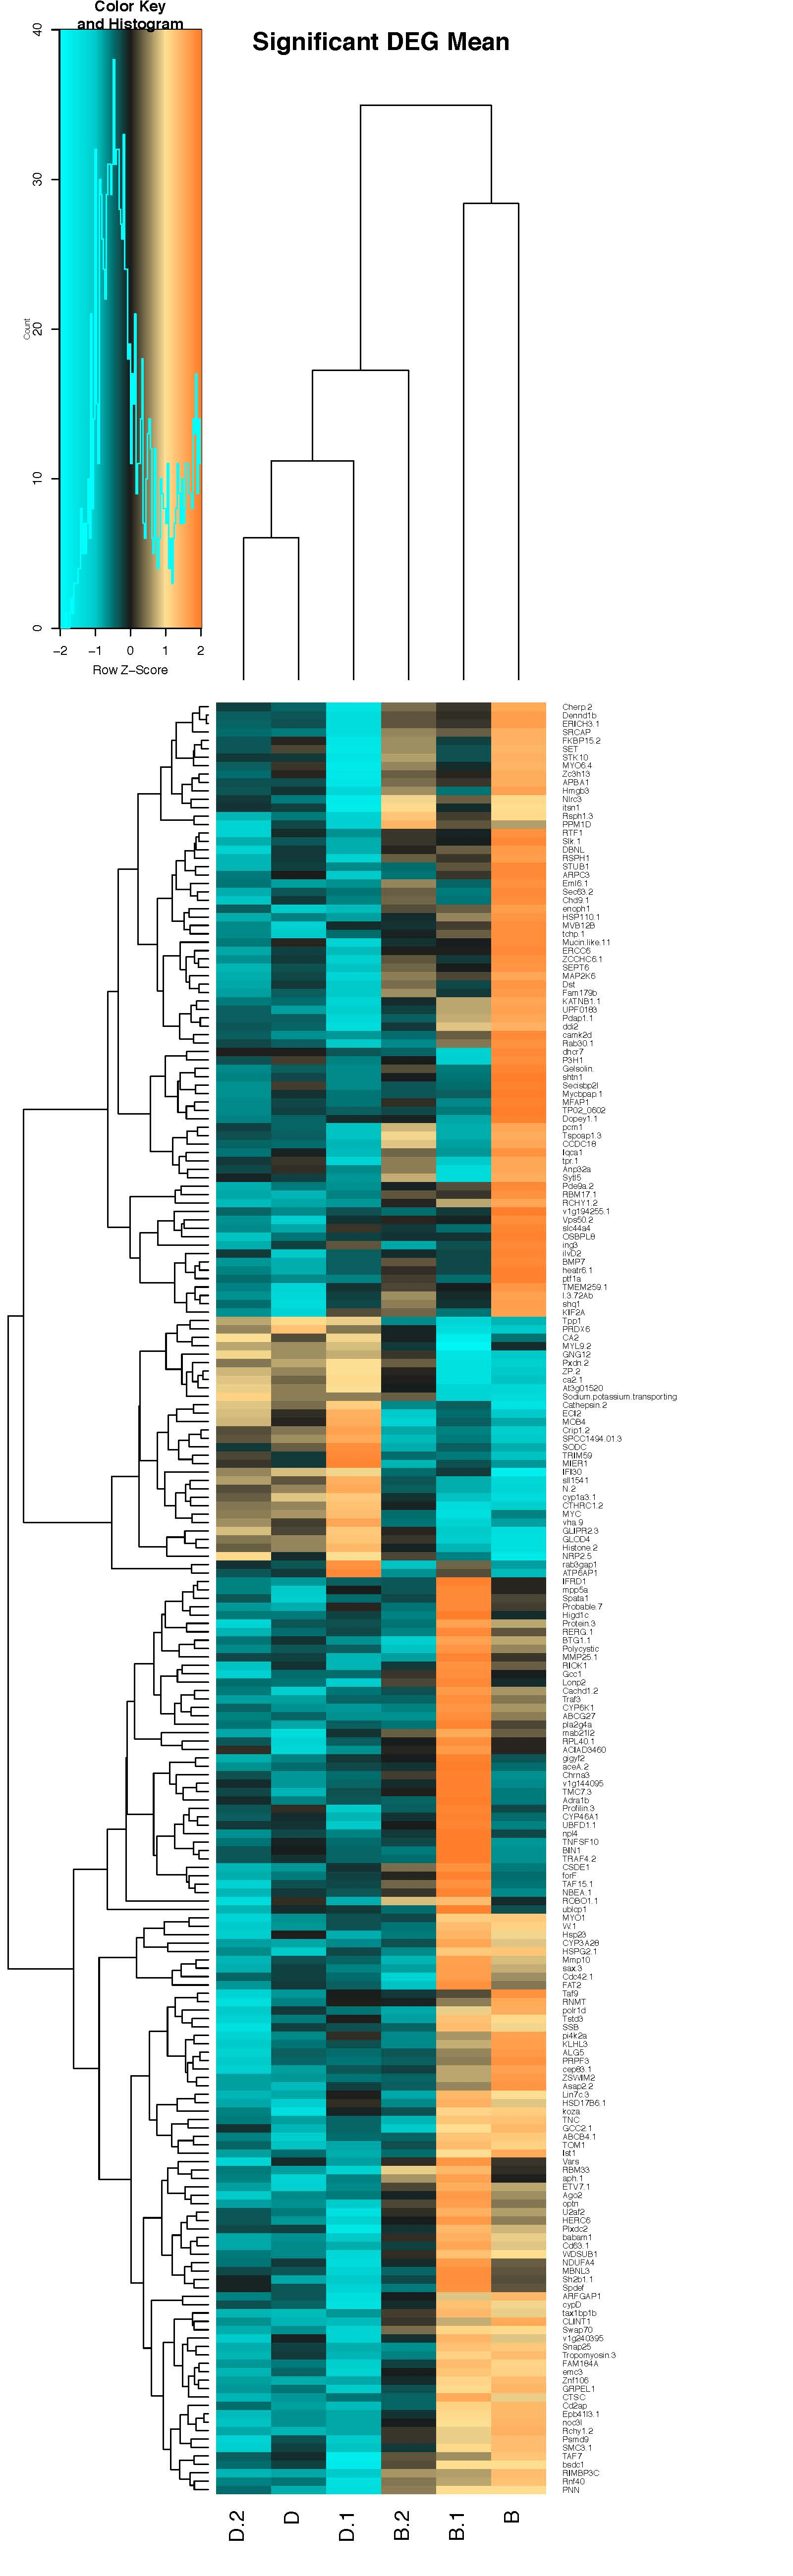
\includegraphics{Ofav 0.5 Sig DEG Mean Heatmap.jpg}

\begin{itemize}
\tightlist
\item
  MAIN FINDINGS:
\item
  From GO MWU analysis of ranked GO term enrichment, we found that
  Postitive Regulation of Cell Proliferation and various Oxidoreductase
  activities are enriched in samples hosting D compared to B recruits
\item
  From analysis of all significantly differentially expressed genes, we
  identified the following:
\item
  SODC (superoxide dismutase) is strongly upregulated in coral hosting D
  compared to B; SODC is an NF-kB response gene; this is consistent with
  our expectations that coral hosting D would perform better under
  thermal/oxidative stress because increased SOD means an increased
  ability to deal with oxidative stress
\item
  To a lesser extent, HSP110 may be downregulated in D compared to B,
  but this may be an effect of count value
\item
  TNFSF10 and TRAF4.2 were identified as upregulated in one B (B.1)
  compared to D (i.e., downregulated in D), but again, this may be an
  effect of count size
\end{itemize}

\end{document}
